%\PassOptionsToPackage{svgnames}{xcolor}
\documentclass[oneside]{book}

\usepackage{geometry}

\usepackage{tcolorbox}
\usepackage{amsmath, amssymb, amsthm}
\usepackage{pdfpages}
\usepackage{sectsty}
\usepackage{multicol}
\usepackage{enumitem}
\usepackage{bm}
\usepackage{caption}
\usepackage{subcaption}
\usepackage{algpseudocode}
\usepackage{algorithm}
\usepackage{mathtools}

\chapterfont{\centering}

%\geometry{top=2cm, left=2cm, bottom=2cm, right=2cm}

%\usepackage{hyphenat}
%\hyphenation{ма-те-ма-ти-ка вос-ста-нав-ли-вать}
%\usepackage[utf8]{inputenc, vietnam}
\usepackage[T2A]{fontenc}
\usepackage[russian, vietnam]{babel}

\definecolor{green}{rgb}{0.0, 255.0, 0.0}
\definecolor{cyan}{rgb}{0.0, 255.0, 255.0}
\definecolor{red}{rgb}{255.0, 0.0, 0.0}
\definecolor{magenta}{rgb}{255.0, 0.0, 255.0}
\definecolor{yello}{rgb}{255.0, 255.0, 0.0}
\definecolor{white}{rgb}{255.0, 255.0, 255.0}

\geometry{a5paper}

\theoremstyle{definition}
\newtheorem{definition}{Định nghĩa}[chapter]
\newtheorem{theorem}{Định lý}[chapter]
\newtheorem{corollary}{Hệ quả}[chapter]
\newtheorem{lemma}{Bổ đề}[chapter]

\newtheorem*{remark}{Nhận xét}
\newtheorem*{axiom}{Tiên đề}
\newtheorem*{example}{Ví dụ}

\renewcommand*\contentsname{Mục lục}

\newcommand{\rank}{\text{rank}}
\newcommand{\RR}{\mathbb{R}}
\newcommand{\ZZ}{\mathbb{Z}}
\newcommand{\QQ}{\mathbb{Q}}
\newcommand{\lcm}{\text{lcm}}

\newenvironment{myexampleblock}[1]{%
    \tcolorbox[colback=LightGreen,colframe=DarkGreen,title=#1]}
    {\endtcolorbox}

\newenvironment{defblock}[2]{%
    \tcolorbox[colback=white,colframe=blue
    ,title=#1
    ]}
    {\endtcolorbox}

\newenvironment{theoremblock}[2]{%
    \tcolorbox[colback=white,colframe=magenta
    ,title=#1
    ]}
    {\endtcolorbox} 

\title{Nơi huyền thoại lưu danh}   
\author{Lê Quốc Dũng} 
\date{\today}

\begin{document}

%=========================================
\begin{titlepage}
		\centering{
			{\fontsize{40}{48}\selectfont 
			Nơi huyền thoại lưu danh}
		}\\
			
		\vspace{10mm}
		\centering{\Large{Lê Quốc Dũng}}\\
		\vspace{\fill}
		\centering \large{2023}
\end{titlepage}

\newpage
%\thispagestyle {empty}

\vspace*{2cm}

\begin{center}
	{\Large 
			\textit{Đường đi ngàn dặm, bắt đầu bằng một bước chân.}
	}
	\Large{\parbox{10cm}{
		\begin{raggedleft}
		\vspace{.5cm}\hfill{Lão Tử}
		\end{raggedleft}
	}
}
\end{center}

\newpage

\tableofcontents

\newpage

\textbf{Bảng các ký hiệu dùng trong sách}

\begin{table}[h]
    \begin{tabular}{c c}
        $\# S$ & số lượng phần tử của tập hợp $S$ (lực lượng của $S$)
    \end{tabular}
\end{table}

\newpage

\part{Đại cương toán học}
\chapter{Đại số cơ bản}

\section{Ánh xạ}

Cho 2 tập hợp $X$ và $Y$. Ánh xạ $f$ biến một phần tử $x \in X$ thành một và chỉ một phần tử $y \in Y$.

Ta ký hiệu
\[f: X \to Y, \; f(x) = y\]

Khi đó, $X$ được gọi là tập nguồn (domain) và $Y$ là tập đích (image).

Ánh xạ có 3 loại:

\begin{itemize}[noitemsep]
    \item Đơn ánh (Injection): Hai phần tử khác nhau của tập nguồn cho hai ảnh khác nhau. Tức là với mọi $x_1, x_2 \in X$ mà $x_1 \neq x_2$, thì $f(x_1) \neq f(x_2)$
    \item Toàn ánh (Surjection): Mọi phần tử $y \in Y$ đều có ít nhất một phần tử $x \in X$ mà $f(x) = y$. Nói cách khác với mỗi phần tử trong $Y$ ta đều tìm được phần tử thuộc $X$ biến thành nó
    \item Song ánh (Injection): Nếu ánh xạ đó vừa là đơn ánh, vừa là toàn ánh
\end{itemize}

\begin{remark}
    Dựa vào định nghĩa và hình vẽ, ta có thể rút ra kết luận như sau
    \begin{itemize}[noitemsep]
        \item Đối với đơn ánh, do mọi phần tử của $X$ đều có ảnh ở $Y$, tuy nhiên có thể có phần tử ở $Y$ không do phần tử nào của $X$ biến thành (trong hình là 5). Do đó $| X | \leq | Y |$
        \item Đối với toàn ánh, mọi phần tử của $Y$ đều có nguồn gốc xuất xứ, tuy nhiên có thể có phần tử của $X$ không biến thành $y$ nào của $Y$ (trong hình là $e$). Do đó $| X | \geq | Y |$
        \item Đối với song ánh, do là kết hợp giữa đơn ánh và toàn ánh, khi đó dấu đẳng thức xảy ra, $| X | = | Y |$
    \end{itemize}
\end{remark}

\begin{figure}[ht]
    \centering
    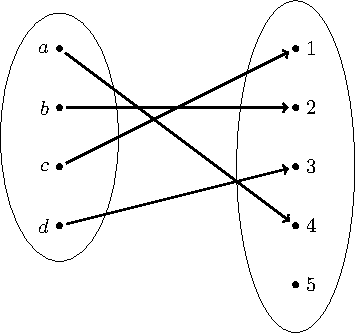
\includegraphics{pics/maps/injection.pdf}
    \caption{Đơn ánh}
\end{figure}

\begin{figure}[ht]
    \centering
    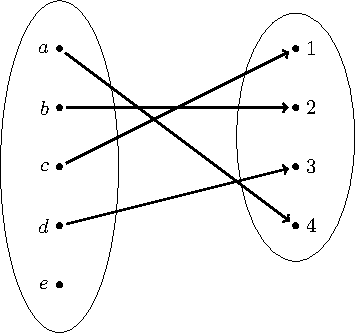
\includegraphics{pics/maps/surjection.pdf}
    \caption{Toàn ánh}
\end{figure}

\begin{figure}[ht]
    \centering
    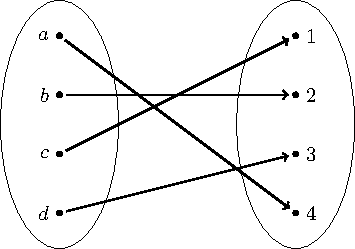
\includegraphics{pics/maps/bijection.pdf}
    \caption{Song ánh}
\end{figure}

\section{Hàm số}

Khi 2 tập nguồn và đích của ánh xạ là 2 tập hợp số, ta có hàm số.

\begin{example}
    Hàm số $f: \RR \rightarrow \RR$ với $y = f(x) = x^3 + x + 1$. Ở đây $X \equiv \RR$ và $Y \equiv \RR$.
\end{example}

Lưu ý rằng tập nguồn và đích không nhất thiết là tập hợp số cơ bản ($\QQ, \RR$) mà cũng có thể là tích Descartes của chúng.

\begin{example}
    Hàm số $f: \RR \times \RR \rightarrow \RR$ với $z = f(x, y) = x + y + xy$. Ở đây $X \equiv \RR$, $Y \equiv \RR$ và $Z \equiv \RR$.
\end{example}

Chúng ta còn một cách gọi khác cho đơn ánh, toàn ánh, song ánh trong tiếng Anh.

\begin{table}[ht]
    \centering
    \begin{tabular}{| l | l | l |}
        \hline
        đơn ánh & injection & one-to-one map \\
        \hline
        toàn ánh & surjection & onto map \\
        \hline
        song ánh & bijection & one-to-one and onto map \\
        \hline
    \end{tabular}

    \caption{Thuật ngữ tiếng Anh cho ánh xạ}
\end{table}

\begin{example}
    Hàm số $f: \RR \rightarrow \RR$ cho bởi $y = f(x) = x^3$ là song ánh.

    \begin{proof}
        Ta thấy nếu $f(x_1) = f(x_2)$, tương đương $x_1^3 = x_2^3$ nên $x_1 = x_2$. Do đó $f$ là đơn ánh.

        Với mọi $y = x^3 \in \RR$, do căn bậc 3 luôn tồn tại nên ta có $x = \sqrt[3]{y}$. Nghĩa là luôn tồn tại $x$ để $f(x) = y$ với mọi $y \in \RR$. Do đó $f$ là toàn ánh.

        Kết luận $f$ là song ánh.
    \end{proof}
\end{example}


\chapter{Mở đầu về số học}

Số học xuất hiện từ xa xưa, từ những bước đi đầu tiên của con
người. Tuy nhiên số học lại mang vẻ bí ẩn khó tưởng, sự phức
tạp vượt ra phạm vi số học. Nhà toán học vĩ đại Gauss từng nói
\textit{Toán học là vua của các môn khoa học, và số học là
nữ hoàng}. Hay một trong 23 bài toán thế kỷ của Hilbert về sự
phi mâu thuẫn của số học, người ta đã chứng minh được rằng
không thể chứng minh sự phi mâu thuẫn của số học chỉ bằng các
lý thuyết về số học.

\section{Phép chia Euclid}

Đây là nền tảng, cơ sở của số học. Từ khi biết tới phép chia
hai số nguyên, ta có thể tìm \textit{thương} và \textit{số dư}.
Nói theo toán học, nếu ta có 2 số nguyên dương $a$ và $b$, thì
tồn tại cặp số $q$, $r$ sao cho $a = qb + r$ với $0 \leq r < b$.

Khi đó, $a$ gọi là số bị chia, $b$ gọi là số chia, $q$ là thương
(q trong quotient) và $r$ là số dư (r trong remainder).

Đặc biệt là sự tồn tại của cặp số $q$ và $r$ là duy nhất. Thật
vậy, nếu ta giả sử tồn tại 2 cặp số $(q_1, r_1)$ và $(q_2, r_2)$ 
đều thỏa đẳng thức trên, nghĩa là
\[a = q_1 b + r_1, \quad a = q_2 b + r_2\]

Trừ 2 đẳng thức vế theo vế ta có $(q_1 - q_2) b + (r_1 - r_2) = 0$.
Tương đương $(r_2 - r_1) = (q_1 - q_2) b$, mà $0 \leq r_1, r_2 < b$
nên $-b < r_2 - r_1 < b$. Như vậy chỉ có thể xảy ra trường hợp
$r_2 - r_1 = 0$ hay $r_2 = r_1$, kéo theo $q_1 = q_2$.

\section{Thuật toán Euclid}

Dựa trên phép chia Euclid, ta có một thuật toán hiệu quả để tìm
ước chung lớn nhất giữa hai số $a$ và $b$.

Ký hiệu $\gcd(a, b)$ là ước chung lớn nhất của $a$ và $b$. Chúng 
ta thực hiện đệ quy như sau:
\[\gcd(a, b) = \begin{cases}
    a, \quad & \text{nếu}\,b = 0 \\
    \gcd(b, a \bmod b), \quad & \text{nếu}\,b \neq 0
\end{cases} 
    \]

Điểm quan trọng ở thuật toán Euclid là thuật toán chắc chắn sẽ dừng
sau một số hữu hạn bước, và kết quả sẽ là ước chung lớn nhất của 2
số $a$ và $b$.
<<<<<<< HEAD
=======

>>>>>>> tuyetngan
\chapter{Lý thuyết nhóm}

Câu chuyện bắt đầu vào một ngày khi mình vẫn còn sống ngày tháng tươi đẹp.

Cho tới khi học \textbf{lý thuyết nhóm} thì đời bớt đẹp hơn tí.

Để bắt đầu mình cần hiểu nhóm là gì.

\section{Nhóm}

%\begin{defblock}{Nhóm (Group)}
\begin{definition}[Nhóm (Group)]
    Một tập hợp $G$ và toán tử 2 ngôi $\star$ trên $G$ tạo thành một nhóm nếu:
    \begin{enumerate}[noitemsep]
        \item Tồn tại phần tử $e \in G$ sao cho với mọi $g \in G$ thì $g \star e = e \star g = g$. Khi đó $e$ được gọi là \textbf{phần tử đơn vị} của $G$.
        \item Với mọi $g \in G$, tồn tại $g' \in G$ sao cho $g \star g' = g' \star g = e$. Khi đó $g'$ được gọi là \textbf{phần tử nghịch đảo} của $g$.
        \item Tính kết hợp: với mọi $a, b, c \in G$ thì $a \star (b \star c) = (a \star b) \star c$.
    \end{enumerate}
\end{definition}

%\end{defblock}

%\begin{defblock}{Nhóm Abel}
\begin{definition}[Nhóm Abel]
    Nếu nhóm $G$ có thêm tính giao hoán, tức là với mọi $a, b \in G$ thì $a \star b = b \star a$ thì $G$ gọi là nhóm giao hoán hay nhóm Abel
\end{definition}
%\end{defblock}

Lý thuyết nhóm thuộc toán trừu tượng, và nó trừu tượng thật. Tuy nhiên khi học về nó mình dần hiểu hơn về cách toán học vận hành và phát triển.

\begin{example}
    Xét tập hợp số nguyên $\ZZ$ và phép cộng 2 số nguyên.
    \begin{enumerate}[noitemsep]
        \item Phần tử đơn vị là 0 vì với mọi $a \in \ZZ$ thì $a + 0 = 0 + a = a$
        \item Với mọi $a \in \ZZ$, phần tử nghịch đảo là $-a$ vì $a + (-a) = (-a) + a = 0$
        \item Phép cộng số nguyên có tính kết hợp do đó thỏa mãn điều kiện về tính kết hợp
    \end{enumerate}
    Như vậy $(\ZZ, +)$ tạo thành nhóm. Lưu ý do phép cộng 2 số nguyên có tính giao hoán nên đây cũng là nhóm Abel.
\end{example}

\begin{example}
    Xét tập hợp số hữu tỉ khác 0 $\QQ^*$ và phép nhân 2 số hữu tỉ. Ta thấy do $a, b \in \QQ^*$ nên tích $a \cdot b$ cũng khác 0, do đó cũng thuộc $\QQ^*$.
    \begin{enumerate}[noitemsep]
        \item Phần tử đơn vị là 1 vì với mọi $a \in \QQ^*$ thì $a \cdot 1 = 1 \cdot a = a$
        \item Với mọi $a \in \QQ^*$, phần tử nghịch đảo là $\frac{1}{a}$ vì $a \cdot \frac{1}{a} = \frac{1}{a} \cdot a = 1$
        \item Phép nhân 2 số hữu tỉ có tính giao hoán do đó thỏa mãn điều kiện về tính kết hợp
    \end{enumerate}
    Tương tự như nhóm $\mathbb{Z, +}$, nhóm $(\QQ^*, \cdot)$ cũng là nhóm Abel.
\end{example}

\section{Nhóm con}

\begin{definition}[Nhóm con (Subgroup)]
    Cho nhóm $(G, \star)$. Tập hợp $H \subset G$ được gọi là \textit{nhóm con} của $G$ nếu với mọi $a, b \in H$ thì $a \star b \in H$
\end{definition}
 
Nghĩa là toán tử $\star$ đóng với các phần tử trong $H$.

\begin{example}
    Xét nhóm $(\ZZ, +)$ như trên. Ta xét tập con gồm các số chẵn của nó
    \[2\ZZ = \{\ldots, -4, -2, 0, 2, 4, \ldots\}\]

    Ta thấy rằng tổng 2 số chẵn vẫn là số chẵn, nghĩa là phép cộng số nguyên đóng trên $2\ZZ$.
    Do đó $(2\ZZ, +)$ là nhóm con của $(\ZZ, +)$.

    Như vậy mọi tập hợp có dạng $n \ZZ$ đều là nhóm con của $(\ZZ, +)$.
\end{example}

\section{Coset}

\begin{definition}[Coset]
    (tạm dịch - \textit{lớp kề} theo wikipedia) Cho nhóm $G$ và nhóm con $H$ của $G$.

    Coset trái của $H$ đối với phần tử $g \in G$ là tập hợp
    \[gH = \{gh : h \in H \}\]

    Tương tự, coset phải là tập hợp
    \[Hg = \{hg : h \in H \}\]
\end{definition}

Từ đây nếu không nói gì thêm ta ngầm hiểu là coset trái.

Ví dụ với nhóm con $2\ZZ$ của $\ZZ$, ta thấy rằng

\begin{enumerate}
    \item Nếu $g \in \ZZ$ là lẻ thì khi cộng với bất kì phần tử nào của $2\ZZ$ ta có số lẻ
    \item Nếu $g \in \ZZ$ là chẵn thì khi cộng với bất kì phần tử nào của $2\ZZ$ ta có số chẵn
\end{enumerate}

Nói cách khác, coset của $2\ZZ$ chia tập $\ZZ$ thành
\[0 (2\ZZ) = \{\ldots, -4, -2, 0, 2, 4, \ldots\}\]
 
\[1 (2\ZZ) = \{\ldots, -3, -1, 1, 3, \ldots \}\]

Trực quan mà nói, 2 coset trên rời nhau.

\begin{remark}
    Hai coset bất kì hoặc rời nhau, hoặc trùng nhau.
\end{remark}

\begin{proof}
    Nếu hai coset rời nhau thì không có gì phải nói. Ta chứng minh trường hợp còn lại.

    Giả sử $g_1 H \cap g_2 H \neq \emptyset$. Như vậy tồn tại $h_1, h_2 \in H$ mà $g_1 h_1 = g_2 h_2$.

    Do $h_1^{-1} \in H$, ta có $g_1 = g_2 h_2 h_1^{-1}$, nghĩa là $g_1 \in g_2 H$.

    Mà mọi phần tử trong $g_1 H$ có dạng $g_1 h$ nên $g_1 h = g_2 h_2 h_1^{-1} h$. Do $H$ là nhóm con của $G$ nên $h_2 h_1^{-1} h \in H$.
    Từ đó $g_1 H \subseteq g_2 H$. Tương tự ta cũng có $g_2 H \subseteq g_1 H$. Vậy $g_1 H = g_2 H$.
\end{proof}

\section{Normal Subgroup}

\begin{definition}[Normal Subgroup]
    (tạm dịch - \textit{nhóm con chuẩn tắc}) Nhóm con $H$ của $G$ được gọi là \textit{normal subgroup} nếu với mọi $g \in G$ ta có coset trái trùng với coset phải.
    \[gH = Hg \; \forall g \in G\]
\end{definition}

Nếu $H$ là normal subgroup của $G$ ta ký hiệu $H \triangleleft G$.

\begin{definition}[Quotient Group]
    (tạm dịch - \textit{nhóm thương}, hay Factor Group - \textit{nhóm nhân tử}). Với nhóm $G$ và normal subgroup của nó là $H$.
    Quotient Group được ký hiệu là $G / H$ và được định nghĩa là tập hợp các coset tương ứng với normal subgroup $H$.
    \[G / H = \{gH : g \in H \}\]

    Ta thấy rằng điều này chỉ xảy ra nếu $H$ là normal subgroup.
\end{definition}

\begin{example}
    Với nhóm $\ZZ$ và normal subgroup của nó là $2\ZZ$.
    Ta thấy $\ZZ / 2 \ZZ = \{0 + 2 \ZZ, 1 + 2 \ZZ\}$
\end{example}
\chapter{Lý thuyết vành}

\section{Vành}

\begin{definition}[Vành (Ring)]
    Cho tập hợp $R$, trên đó ta định nghĩa 2 toán tử \textit{cộng} và \textit{nhân}.

    Khi đó, $(R, +, \times)$ tạo thành vành nếu

    \begin{itemize}
        \item $(R, +)$ là nhóm Abel
        \item $(R, \times)$ có tính kết hợp với phép nhân. Với mọi $a, b, c \in R$ thì $a \times (b \times c) = (a \times b) \times c$
        \item Tính phân phối của phép cộng và phép nhân. Với mọi $a, b, c \in R$ thì $(a + b) \times c = a \times c + b \times c$
    \end{itemize}
\end{definition}

Tóm lại, $(R, +, \times)$ là vành nếu nó là nhóm Abel đối với phép cộng và có tính kết hợp với phép nhân.

\textbf{Lưu ý}. Phép nhân ở đây không nhất thiết có phần tử đơn vị, hay phần tử nghịch đảo như trong định nghĩa nhóm. Trong trường hợp này $(R, \times)$ gọi là semigroup (nửa nhóm).

\begin{definition}[Vành với đơn vị - Ring with identity] Nếu có phần tử $1_R \neq 0_R \in R$ sao cho với mọi $r \in R$ ta đều có
    \[1_R \times r = r \times 1_R = r\]
    thì $1_R$ được gọi là phần tử đơn vị đối với phép nhân.
\end{definition}

Ta thường ký hiệu $0_R$ là phần tử đơn vị của phép cộng $(R, +)$ và gọi là \textbf{phần tử trung hòa}.
Khi đó phần tử nghịch đảo của phép cộng gọi là \textbf{phần tử đối} và được ký hiệu là $-a$ nếu là đối của phần tử $a$.

Và $1_R$ là \textbf{phần tử đơn vị} đối với phép nhân $(R, \times)$.

\begin{definition}[Vành giao hoán - Commutative ring]
    Nếu ta có tính giao hoán đối với phép nhân, nghĩa là với mọi $a, b \in $ đều thỏa
    \[a \times b = b \times a\]
    thì ta nói là vành giao hoán (không cần nói rõ là phép nhân vì phép cộng bắt buộc phải giao hoán theo định nghĩa vành rồi).
\end{definition}

\section{Ideal}

\begin{definition}[Ideal]
    Xét vành $(R, +, \times)$. Một tập con $I$ của $R$ được gọi là 
    \textit{ideal trái} nếu
    \begin{itemize}
        \item $(I, +)$ là nhóm con của $(R, +)$
        \item với mọi $r \in R$, với mọi $x \in I$ thì $rx \in I$
    \end{itemize}
\end{definition}

Ta định nghĩa tương tự với ideal phải, khi đó $xr \in I$.
Từ đây về sau nếu không nói gì thêm nghĩa là mình xét ideal trái.

\begin{definition}[Ideal chính - Principal ideal]
    Nếu $I = aR$ với $a$ là phần tử nào đó trong $R$ thì $I$ được gọi 
    là  \textit{principal ideal}.
\end{definition}

Nói cách khác, nếu có một phần tử trong $R$ "sinh" ra được $I$ thì 
$I$ là principal.

\begin{definition}[Ideal cực đại - Maximal ideal]
    Nếu $I$ là một ideal của $R$ và không tồn tại tập con $I'$ mà 
    $I \subset I' \subset R$ (tập con thực thụ) thì $I$ được gọi
    là maximal ideal.
\end{definition}

\begin{corollary}
    Xét vành số nguyên $\ZZ$. Khi đó mọi ideal của $\ZZ$ đều là principal.
\end{corollary}

\begin{proof}
    Giả sử ideal $I$ của $\ZZ$ có phần tử dương nhỏ nhất là $n$.
    Theo định nghĩa của ideal thì với mọi $q \in \ZZ$ ta có 
    $qn \in I$.

    Nếu phần tử $a \in I$, theo phép chia Euclid ta có $a = qn + r$
    với $0 \leq r < n$, mà $a \in I$ và $qn \in I$ nên $r = a - qn \in I$.
    Tuy nhiên phần tử dương nhỏ nhất thuộc $I$ là $n$, do đó $r = 0$.

    Nói cách khác mọi phần tử $a \in I$ đều có dạng $qn$ với $q \in \ZZ$.

    Vậy mọi ideal đều là principal.
\end{proof}

\begin{corollary}
    Ideal $I$ của $\ZZ$ là maximal khi và chỉ khi $I = n\ZZ$ với
    $n$ là số nguyên tố.
\end{corollary}

\begin{proof}
    Ta chứng minh chiều thuận, chiều ngược tương tự. Sử dụng phản chứng,
    ta giả sử $n$ là hợp số. Khi đó $n = n_1 n_2$ ($n_1 \geq n_2 > 1$).

    Khi đó $n \ZZ \subset n_1 \ZZ \subset \ZZ$, suy ra ideal không phải
    maximal. Ta có điều phải chứng minh.
\end{proof}
\chapter{Tác động nhóm}

Tác động nhóm (Group Action) cho phép chúng ta đếm những cấu hình tổ hợp mà việc vét cạn rồi loại bỏ sẽ tốn nhiều công sức cũng như sai sót.

\section{Tác động nhóm}

Cho tập hợp $M$ và nhóm $G$. Ta nói $G$ \textit{tác động trái} lên $M$ với ánh xạ:
\[\alpha: G \times M \rightarrow M\]
thỏa mãn 2 tiên đề sau:

\begin{itemize}[noitemsep]
    \item Identity: $\alpha (e, m) = m$ với mọi $m \in M$
    \item Compatibility: $\alpha (g, \alpha (h, m)) = \alpha (g h, x)$
\end{itemize}

Ta thường ký hiệu $\alpha (g, m)$ bởi $g(m)$ hay thậm chí đơn giản hơn là $gm$. Ký hiệu $gm$ sẽ được sử dụng từ đây về sau.

Khi đó 2 tiên đề trên tương đương với:

\begin{itemize}[noitemsep]
    \item Identity: $e m = m$ với mọi $m \in M$
    \item Compatibility: $g(hm) = (gh)m$ với mọi $m \in M$ và $g, h \in G$
\end{itemize}

\begin{definition}[Stabilizer]
    (tạm dịch - \textit{nhóm con ổn đinh}). Với phần tử $m \in M$, tập hợp các phần tử $g \in G$ mà $gm = m$ được gọi là nhóm con ổn định của nhóm $G$. Ta ký hiệu
    \[G_m = \{ g \in G : gm = m \}\]
\end{definition}

\begin{definition}[Orbit]
    (tạm dịch - \textit{quỹ đạo}) của phần tử $m \in M$ là tập hợp
    \[G(m) = \{gm : g \in G\}\]
\end{definition}

\begin{remark}
    Hai orbit của hai phần tử bất kì hoặc rời nhau, hoặc trùng nhau.
\end{remark}

\begin{proof}
    Giả sử ta có $m_1, m_2 \in M$ mà $G(m_1) \cap G(m_2) \neq \emptyset$.

    Khi đó tồn tại $g_1, g_2 \in G$ để $g_1 m_1 = g_2 m_2$. Suy ra $m_1 = g_1^{-1} g_2 m_2$.

    Mà mọi phần tử trong $G(m_1)$ có dạng $g m_1$ nên $g m_1 = g g_1^{-1} g_2 m_2$ nên $G(m_1) \subseteq G(m_2)$.

    Chứng minh tương tự ta cũng có $G(m_2) \subseteq G(m_1)$ nên $G(m_1) \equiv G(m_2)$.
\end{proof}

\begin{corollary}
    Tập hợp $M$ là giao của các orbit rời nhau. Giả sử ta có $t$ orbit rời nhau $G(m_1), G(m_2), \ldots, G(m_t)$ thì
    \[M = G(m_1) \cup G(m_2) \cup \ldots \cup G(m_t)\]
\end{corollary}

\begin{example}
    Cho nhóm $\mathcal{S}_3$ có 6 phần tử $(1)(2)(3)$, $(1)(2,3)$, $(2)(1,3)$, $(3)(1,2)$, $(1,2,3)$, $(1,3,2)$.

    Xét tập hợp $M = \{1, 2, 3\}$. Khi đó, xét từng hoán vị trên, ta có:
    \[G_1 = \{(1)(2)(3), (1)(2,3)\}\]
    và
    \[G(1) = \{ 1, 2, 3 \}\]
\end{example}

Ta nhận thấy $G(1) = G(2) = G(3)$, và $\lvert G \rvert = 6 = \lvert G_1 \rvert \cdot \lvert G(1) \rvert$

Hay nói cách khác, $\lvert G(m) \rvert = [G: G_m]$ với $G_m$ là stabilizer của phần tử $m$ và $[G: G_m]$ là subgroup index của $G_m \subset G$, và bằng $\frac{\lvert G \rvert}{\lvert G_m \rvert}$ nếu là nhóm hữu hạn.

\begin{definition}
    Hai phần tử $m, n \in M$ được gọi là \textit{có quan hệ} với nhau dưới tác động của nhóm $G$ nếu tồn tại phần tử $g \in G$ sao cho $m = g n$.
    Ta ký hiệu là $m \tilde{G} n$.
\end{definition}

\begin{remark}
    Quan hệ được định nghĩa như trên là quan hệ tương đương.
\end{remark}

\begin{proof}
    Ta cần chứng minh quan hệ trên có tính phản xạ, đối xứng và bắc cầu.
    
    1. Tác động nhóm phải thỏa mãn $e m = m$ với mọi $m \in M$. Do đó có tính phản xạ.

    2. Với mọi $m, n$ mà $m \tilde{G} n$ thì tồn tại $g \in G$ mà $m = gn$. Do tồn tại $g^{-1} \in G$, nhân cho 2 vế ta có $g^{-1} m = n$, nghĩa là
    $n \tilde{G} m$. Vậy quan hệ này có tính đối xứng.

    3. Nếu $m \tilde{G} n$ và $n \tilde{G} p$ thì tồn tại 2 phần tử $g_1, g_2 \in G$ mà $m = g_1 n$ và $n = g_2 p$.
    Suy ra $m = g_1 g_2 p$, tương đương $m \tilde{G} p$, do đó có tính bắc cầu.
\end{proof}

\section{Bổ đề Burnside}

Các trạng thái khác nhau của tập hợp $M$ có thể là \textit{tương đương} nhau nếu chúng nằm trong cùng lớp tương đương dưới tác động của nhóm $G$.

Bổ đề Burnside cho phép chúng ta tính được số trạng thái khác nhau (hay cấu hình khác nhau) mà chúng ta dễ bị nhầm lẫn hoặc bỏ sót trong quá trình vét cạn.

Bài tập về bổ đề Burnside và định lý Polya được tham khảo tại \cite{Tarannikov}.

\begin{lemma}[Bổ đề Burnside]
    Với nhóm $G$ tác động lên tập hợp $M$, ta có:
    \[t_G = \frac{1}{\lvert G \rvert} \sum_{g \in G} \lvert M^g \rvert \]
    trong đó, $t_G$ là số lớp tương đương của tập $M$ dưới tác động của nhóm $G$

    $\lvert M^g \rvert$ là số điểm bất động của tập $M$ dưới tác động của phần tử $g$, nghĩa là $M^g = \{ m \in M : gm = m\}$.
\end{lemma}

\section{Ví dụ bài toán đếm sử dụng bổ đề Burnside}

\begin{example}
    Cho hình tứ diện đều. Ta tô 4 đỉnh của nó bằng 3 màu xanh, đỏ, vàng. Hỏi có bao nhiêu cách tô như vậy?

    Ta cần lưu ý một điều, 2 cách tô là tương đương nhau (giống nhau) nếu tồn tại một phép quay các đỉnh biến cách tô này thành cách tô kia.

    \begin{figure}[ht]
        \centering
        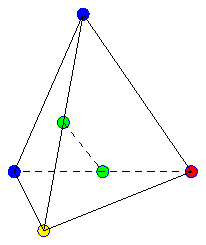
\includegraphics{pics/tetrahedron/tetrahedron1.pdf}
        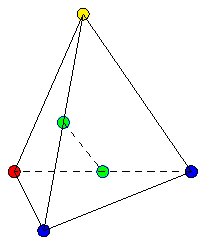
\includegraphics{pics/tetrahedron/tetrahedron2.pdf}
        \caption{Phép quay trục tạo bởi trung điểm hai cạnh đối nhau}
    \end{figure}

    Như hình trên ta thấy nếu chọn trục quay là đường thẳng nối trung điểm 2 cạnh đối diện (2 điểm xanh lá) thì đỉnh trên và đỉnh dưới đổi chỗ cho nhau (xanh và vàng), đỉnh trái và đỉnh phải đổi chỗ cho nhau (xanh và đỏ).

    Ta giải bài này như sau:

    Đầu tiên ta đánh số các đỉnh của tứ diện (như hình)

    \begin{figure}[ht!]
        \centering
        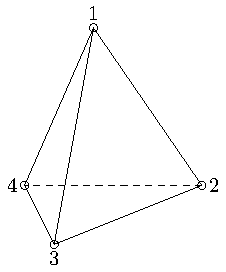
\includegraphics{pics/tetrahedron/tetrahedron3.pdf}
        \caption{Đánh số hình}
    \end{figure}
    
    Ta có 3 trường hợp biến đổi sau:

    \underline{Trường hợp 1}. Giữ nguyên 1 đỉnh và trục quay là đường thẳng đi qua đỉnh đó và tâm của mặt đối diện.

    \begin{figure}[ht!]
        \centering
        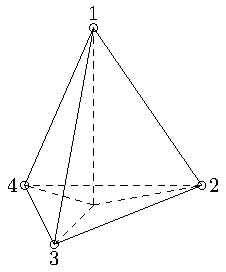
\includegraphics{pics/tetrahedron/tetrahedron4.pdf}
        \caption{Trường hợp 1}
    \end{figure}

    Khi đó phép quay (ngược chiều đồng hồ) tương ứng hoán vị $(1)(2,3,4)$ (quay 60 độ) và $(1)(2,4,3)$ (quay 120 độ).

    Do ta chọn 1 đỉnh cố định thì ta có 4 cách chọn, và với mỗi cách chọn đỉnh cố định ta có thể quay 2 cách nên ta có tổng là 8 hoán vị.

    \underline{Trường hợp 2}. Ta chọn trung điểm 2 cạnh đối nhau và nối lại thành trục quay như hình trong ví dụ. Khi đó tương ứng với hoán vị $(1,4)(2,3)$.

    Ta có $\frac{C^2_4}{2!} = 3$ hoán vị.

    \underline{Trường hợp 3}. Hoán vị đồng nhất $(1)(2)(3)(4)$.

    Tóm lại, tập hợp $M$ ở đây là tập hợp 4 đỉnh của tứ diện, và nhóm tác động lên $M$ là nhóm con 12 phần tử của $\mathcal{S}_4$.

    Như vậy, ví dụ với hoán vị $(1)(2,3,4)$, nếu ta muốn sau phép quay giữ nguyên trạng thái (hay nói cách khác là tìm $M^g$) thì ta
    tô màu đỉnh 1 tùy ý, đỉnh 2-3-4 chung màu (cũng tùy ý).

    Suy ra ta có $3 \cdot 3$ cách tô. Tương tự với các hoán vị dạng $(1,4)(2,3)$.

    Như vậy $t_G = \frac{1}{12}(1 \cdot 3^4 + 8 \cdot 3^2 + 3 \cdot 3^2) = 15$ cách tô màu khác nhau.
\end{example}

Tổng quát, nếu có $k$ màu thì số lớp tương đương là
\[t_G = \frac{1}{12}(1 \cdot k^4 + 8 \cdot k^2 + 3 \cdot k^2) = \frac{1}{12}(k^4 + 11 k^2)\]

\section{Chỉ số chu trình}

Với mỗi hoán vị trong tập $G$ (theo định lý Cayley thì mọi nhóm hữu hạn đều isomorphism với nhóm con nào đó của nhóm hoán vị), ta viết dưới dạng các chu trình độc lập
\[\underbrace{(g_1) (g_2) \ldots (g_{t_{1}})}_{t_1} \underbrace{(g_{j_1} g_{j_2}) (g_{j_3} g_{j_4})\ldots}_{t_2}\]
Nếu ta viết hoán vị dưới dạng các chu trình rời nhau, ta gọi

\begin{tabular}{c c}
    $t_1$ & là số chu trình có độ dài 1 \\
    $t_2$ & là số chu trình có độ dài 2 \\
    $\ldots$ & tương tự \\
    $t_n$ & là số chu trình có độ dài $n$
\end{tabular}

Khi đó, chỉ số chu trình của hoán vị ứng các biến $z_1, z_2, \ldots, z_n$ là
\[I_g (z_1, z_2, ,\ldots, z_n) = z_1^{t_1} z_2^{t_2} \ldots z_n^{t_n}\]

\begin{example}
Xét hoán vị $(1,2,3)(4)(5)(6,7) \in \mathcal{S}_7$

Ta có 2 chu trình độ dài 1, 1 chu trình độ dài 2 và 1 chu trình độ dài 3.
Không có chu trình độ dài 4, 5, 6, 7.

Do đó chỉ số chu trình là 
\[I_g (z_1, z_2, z_3) = z_1^2 z_2^1 z_3^1\]

\end{example}

\begin{remark}
    Bất kì hoán vị nào thuộc $\mathcal{S}_n$ đều thỏa $1 \cdot t_1 + 2 \cdot t_2 + \ldots + n \cdot t_n = n$.
\end{remark}

\begin{definition}[Cyclic index]
    (tạm dịch - \textit{chỉ số chu trình}) của nhóm G là
    \[P_G (z_1, z_2, \ldots, z_n) = \frac{1}{G}\sum_{g \in G} I_g (z_1, z_2, \ldots, z_n)\]
\end{definition}

Nhìn lại ví dụ về tứ diện bên trên, các đỉnh nằm trong cùng chu trình cần được tô cùng màu. Như vậy mỗi $z_i$ tương ứng với một màu.

Từ đó, với ví dụ trên
\[P_G(z_1, z_2, z_3) = \frac{1}{12}\big(z_1^4 + 8 z_1 z_3 + 3 z_2^2\big)\]

Cho mỗi $z_i = 3$ ta có kết quả phép tính theo bổ đề Burnside.

\section{Định lý Polya}

Định lý Polya là một mở rộng cho bổ đề Burnside, cho phép chúng ta đếm số lớp tương đương thỏa mãn điều kiện nhất định (về số lượng phần tử nhất định nhận trạng thái nhất định).

Ví dụ với hình tứ diện như trên nhưng ta thêm điều kiện tô 2 đỉnh màu vàng, 1 đỉnh màu đỏ và 1 đỉnh màu xanh (không tô tổng quát nữa).

Ta ký hiệu tập $R$ là tập hợp các trạng thái có thể nhận của mỗi phần tử $m \in M$.
\[R = \{r_1, r_2, \ldots, r_c \}\]
Ở ví dụ trên thì $R = \{\text{đỏ}, \text{xanh}, \text{vàng}\}$.

Ta thay mỗi $z_i$ trong chỉ số chu trình bằng tổng $\sum_{r \in R} r^i$.

\begin{example}
    Giả sử ta tô màu 4 đỉnh tứ diện với 2 màu $R = \{r_1, r_2\}$.

    Với $z_1$ ta thay bằng $r_1 + r_2$

    Với $z_2$ ta thay bằng $r_1^2 + r_2^2$

    Với $z_3$ ta thay bằng $r_1^3 + r_2^3$

    Khi đó $P_G$ tương đương với
    \[\frac{1}{12}\big[(r_1 + r_2)^4 + 8 \cdot (r_1 + r_2)(r_1^3 + r_2^3) + 3 \cdot (r_1^2 + r_2^2)^2\big]\]
    Khai triển ra (lưu ý là ở đây không có tính giao hoán phép nhân)
    \begin{align*}
        (r_1 + r_2)^4 = & r_1 r_1 r_1 r_1 + r_1 r_1 r_1 r_2 + r_1 r_1 r_2 r_1 + r_1 r_1 r_2 r_2 \\
        + & r_1 r_2 r_1 r_1 + r_1 r_2 r_1 r_2 + r_1 r_2 r_2 r_1 + r_1 r_2 r_2 r_2 \\
        + & r_2 r_1 r_1 r_1 + r_2 r_1 r_1 r_2 + r_2 r_1 r_2 r_1 + r_2 r_1 r_2 r_2 \\
        + & r_2 r_2 r_1 r_1 + r_2 r_2 r_1 r_2 + r_2 r_2 r_2 r_1 + r_2 r_2 r_2 r_2
    \end{align*}

    Mình thấy rằng có 16 cấu hình khác nhau tương ứng 16 cách tô 2 màu cho 4 đỉnh. Tương tự

    \begin{align*}
        (r_1 + r_2) (r_1^3 + r_2^3) & = r_1^4 + r_1 r_2^3 + r_2 r_1^3 + r_2^4 \\
        & = r_1 r_1 r_1 r_1 + r_1 r_2 r_2 r_2 + r_2 r_1 r_1 r_1 + r_2 r_2 r_2 r_2
    \end{align*}

    và cuối cùng

    \begin{align*}
        (r_1^2 + r_2^2)^2 & = r_1^4 + r_1^2 r_2^2 + r_2^2 r_1^2 + r_2^4 \\
        & = r_1 r_1 r_1 r_1 + r_1 r_1 r_2 r_2 + r_2 r_2 r_1 r_1 + r_2 r_2 r_2 r_2
    \end{align*}

    Việc không có tính giao hoán với phép nhân làm biểu thức cồng kềnh và phức tạp.
    Do đó mình thêm một tập hợp $W$ là vành giao hoán, và xét ánh xạ $w: R \mapsto W$ với $w(r_i) = w_i$.

    Khi đó nếu thay $r_i$ bởi $w_i$ vào bên trên biểu thức sẽ rất đẹp
    \[P_G(w_1, w_2) = \frac{1}{12} \big[(w_1 + w_2)^4 + 8 (w_1 + w_2) (w_1^3 + w_2^3) + 3 (w_1^2 + w_2^2)^2\big]\]

    Khai triển và thu gọn ta có
    \begin{align*}
    P_G(w_1, w_2) & = \frac{1}{12} \big[12 w_1^4 + 12 w_1^3 w_2 + 12 w_1^2 w_2^2 + 12 w_1 w_2^3 + 12 w_2^4\big] \\
    & = w_1^4 + w_1^3 w_2 + w_1^2 w_2^2 + w_1 w_2^3 + w_2^4
    \end{align*}

    Ở đây, định lý Polya nói rằng, số mũ của $w_i$ thể hiện số lượng phần tử của tập $M$ nhận giá trị $r_i$,
    và hệ số trước mỗi toán hạng là số lớp tương đương tương ứng với số lượng phần tử của tập $M$ nhận các giá trị $r_i$.

    Nói cách khác:
    \begin{itemize}[noitemsep]
        \item có 1 lớp tương đương mà 4 đỉnh nhận màu $r_1$
        \item có 1 lớp tương đương mà 3 đỉnh nhận màu $r_1$ và 1 đỉnh nhận màu $r_2$
        \item có 1 lớp tương đương mà 2 đỉnh nhận màu $r_1$ và 2 đỉnh nhận màu $r_2$
        \item có 1 lớp tương đương mà 1 đỉnh nhận màu $r_1$ và 3 đỉnh nhận màu $r_2$
        \item cuối cùng là 1 lớp tương đương mà 4 đỉnh nhận màu $r_2$.
    \end{itemize}
\end{example}

Quay lại vấn đề tô 4 đỉnh tứ diện với 3 màu xanh, đỏ, vàng. Tìm số cách tô 2 đỉnh màu vàng, 1 đỉnh màu đỏ và 1 đỉnh màu xanh.

Đặt $w(\text{vàng}) = x$, $w(\text{đỏ}) = y$ và $w(\text{xanh}) = z$

Ta có
\[P_G = \frac{1}{12} \big[(x + y + z)^4 + 8 \cdot (x + y + z) (x^3 + y^3 + z^3) + 3 \cdot (x^2 + y^2 + z^2)^2\big]\]

Như vậy đề bài tương ứng việc tìm hệ số của hạng tử $x^2 yz$ trong biểu thức trên. Mình tính ra kết quả là 1.
%\chapter{Đại số Boolean}

Boolean (hay luận lý) chỉ giá trị đúng hoặc sai của mệnh đề nào đó. 
Theo cách hiểu cơ bản, boolean gồm 2 giá trị 0 hoặc 1 (sai hoặc đúng).

\section{Hàm Boolean}

Hàm boolean $f$ đối với các biến $x_1, x_2, \ldots, x_n$ là hàm số nhận giá trị trong $\{0, 1\}^n$ và trả về giá trị thuộc $\{0, 1\}$.

Nghĩa là $f: \{0,1\}^n \mapsto \{0, 1\}$

\section{Các loại hàm boolean}

\begin{definition}{Đa thức Zhegalkin}
    Với hàm bool $f(x_1, x_2, \ldots, x_n)$, đa thức Zhegalkin tương ứng với hàm bool đó là cách biểu diễn
    đa thức đó dưới dạng tổng các tích như sau
    \[f(x_1, x_2, \ldots, x_n) = a_0 \oplus a_1 x_1 \oplus a_2 x_2 \oplus a_3 x_1 x_2 \oplus \ldots \oplus a_k x_1 x_2 \ldots x_n\]
    với $a_i \in \{0, 1\}$. Ta thấy rằng có $n$ biến, do đó có $2^n$ hệ số $a_i$.
\end{definition}

\begin{example}
    Cho hàm bool $f(x, y) = x \vee y$. Ta có bảng chân trị sau
    \begin{table}[ht]
        \centering
        \begin{tabular}{c c c}
            $x$ & $y$ & $f(x, y)$ \\
            0 & 0 & 0 \\
            0 & 1 & 1 \\
            1 & 0 & 1 \\
            1 & 1 & 1 \\
        \end{tabular}
    \end{table}
    Bảng chân trị này tương đương với đa thức Zhegalkin
    \[f(x, y) = x \oplus y \oplus xy\]
\end{example}

\chapter{Ba đường Conic}

Ba đường Conic bao gồm ellipse, hyperbol và parabol.

\section{Ellipse}

\begin{defblock}{Ellipse}

    Đường ellipse là tập hợp các điểm sao cho tổng khoảng cách từ nó tới 2 điểm cố định là 1 hằng số.
\end{defblock}

Nghĩa là, với 2 điểm cố định $F_1, F_2$, tập hợp các điểm $M$ sao cho $M F_1 + M F_2 = 2a$ với $a$ là hằng số tạo thành đường ellipse.

Ở trên hệ tọa độ, nếu ta chọn $F_1$ và $F_2$ nằm trên $Ox$ và đối xứng qua $Oy$, tức là $F_1 = (-c, 0)$ và $F_2 = (c, 0)$, thì các điểm $M = (x, y)$ nằm trên ellipse thỏa

$$MF_1 + MF_2 = \sqrt{(x+c)^2 + y^2} + \sqrt{(x-c)^2 + y^2} = 2a$$

Tương ứng với biển đổi thành phương trình

$$\frac{x^2}{a^2} + \frac{y^2}{a^2 - c^2} = 1$$

Đặt $b^2 = a^2 - c^2$ thì phương trình của ellipse trở thành

$$\frac{x^2}{a^2} + \frac{y^2}{b^2} = 1$$

Phương trình này gọi là \textbf{phương trình chính tắc}.

\begin{figure}[ht]
    \centering
    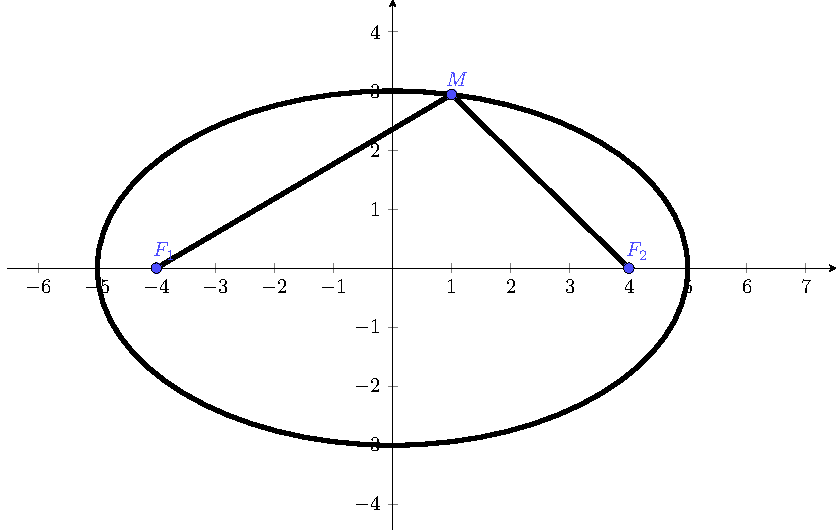
\includegraphics[width=\textwidth]{pics/conics/ellipse.pdf}
    \caption{Ellipse với phương trình $\frac{x^2}{25} + \frac{y^2}{9} = 1$}
\end{figure}

Trong phương trình $$\frac{x^2}{a^2} + \frac{y^2}{b^2} = 1$$

thì $a$ là khoảng cách từ tâm tới 2 biên trái hoặc phải, nên $a$ là \textbf{độ dài bán trục lớn}.

Tương tự, $b$ là \textbf{độ dài bán trục nhỏ} (khoảng cách từ tâm tới 2 biên trên dưới).

Từ cách đặt $b^2 = a^2 - c^2$ tương đương $c^2 = a^2 - b^2$ thì $c$ gọi là \textbf{tiêu cự} của ellipse.

Các điểm $F_1, F_2$ gọi là \textbf{tiêu điểm} của ellipse.

Với ví dụ trên $\frac{x^2}{25} + \frac{y^2}{9} = 1$ thì $a=5, b=3$. Suy ra $c=4$ (lưu ý là $a, b > 0$ và $c \geq 0$).

Các đỉnh nằm ở các tọa độ $(-a, 0), (a, 0), (0, b), (0, -b)$. Các tiêu điểm nằm ở $(-c, 0), (c, 0)$.

\begin{remark}
    Khi $c=0$, tức là 2 tiêu điểm trùng nhau, ta có đường tròn.
\end{remark}

Tâm sai của ellipse là $e = \frac{c}{a} < 1$

\section{Hyperbol}

\begin{defblock}{Hyperbol}

    Đường hyperbol là tập hợp các điểm sao cho giá trị tuyết đối hiệu số khoảng cách từ nó tới 2 điểm cố định là 1 hằng số.
\end{defblock}

Nghĩa là, với 2 điểm cố định $F_1, F_2$, tập hợp các điểm $M$ sao cho $| M F_1 - M F_2 | = 2a$ với $a$ là hằng số tạo thành đường hyperbol.

Ở trên hệ tọa độ, nếu ta chọn $F_1$ và $F_2$ nằm trên $Ox$ và đối xứng qua $Oy$, tức là $F_1 = (-c, 0)$ và $F_2 = (c, 0)$, thì các điểm $M = (x, y)$ nằm trên hyperbol thỏa

$$| MF_1 - MF_2 | = | \sqrt{(x+c)^2 + y^2} - \sqrt{(x-c)^2 + y^2} | = 2a$$

Tương ứng với biển đổi thành phương trình

$$\frac{x^2}{a^2} - \frac{y^2}{a^2 - c^2} = 1$$

Đặt $b^2 = a^2 - c^2$ thì phương trình của hyperbol trở thành

$$\frac{x^2}{a^2} - \frac{y^2}{b^2} = 1$$

Đường hyperbol cắt trục $Ox$ tại 2 điểm $A_1 = (-a, 0)$ và $A_2 = (a, 0)$.

Tiêu điểm của hyperbol ở $F_1 = (-c, 0)$ và $F_2 = (c, 0)$.

Đường hyperbol có 2 tiệm cận là đường thẳng $y = \frac{b}{a} x$ và $y = -\frac{b}{a} x$.

Tâm sai của hyperbol là $e = \frac{c}{a} > 1$.

\section{Parabol}

\begin{defblock}{Parabol}

    Đường parabol là tập hợp các điểm cách đều một điểm cố định và một đường thẳng cố định.

\end{defblock}

\begin{figure}[ht]
    \centering
    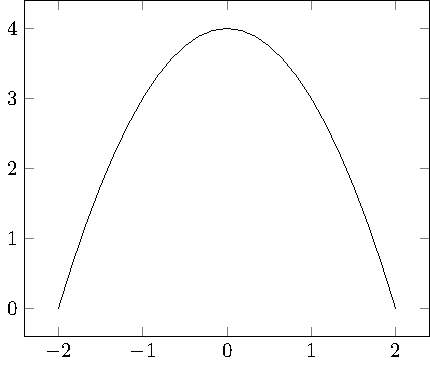
\includegraphics{pics/conics/parabola.pdf}
    \caption{Parabol với phương trình $y = -x^2 + 4$}
\end{figure}

Nghĩa là, với 1 điểm cố định $F$ và đường thẳng cố định $(d)$, parabol là tập hợp các điểm $M$ sao cho $MF = d(M, d)$ với $d(M, d)$ là khoảng cách từ $M$ tới đường thẳng $(d)$.

Phép dời tọa độ cho phép ta dời một hình parabol có đỉnh ở bất kì điểm nào về gốc tọa độ.

Tức là, không mất tính tổng quát, ta chỉ cần xét các parabol dạng $y=ax^2$ là đủ.

Điểm cố định ở trên được gọi là \textbf{tiêu điểm}. Đường thẳng cố định ở trên gọi là \textbf{đường chuẩn}.

Parabol có tính đối xứng nên tiêu điểm nằm trên $Oy$. Đặt tọa độ của nó là $F = (0, f)$.

Đường chuẩn nằm ngang nên ta có parabol là các điểm $M = (x, y)$ sao cho

$MF = \sqrt{x^2 + (y-f)^2}$ và $d(M, d) = y+f$ 
(trường hợp $M$ trùng với đỉnh nên điều kiện của parabol xảy ra tương đương với $M$ cách đều tiêu điểm và đường chuẩn, nghĩa là đường chuẩn có dạng $y=-f$).

Do đó $\sqrt{x^2 + (y-f)^2} = y + f$. Bình phương và biến đổi ta thu gọn được
$$f = \frac{1}{4a}$$

Thường thì ta đặt $p = f$, khi đó phương trình parabol trở thành 
$$x^2 = 4py$$

Đây là dạng chính tắc của parabol với trục đối xứng dọc.

Tâm sai của parabol là $e = \frac{c}{a} = 1$.

\newpage

%$| \mathbb{N} | = | \mathbb{Z} | ?$
%$f: \mathbb{N} \rightarrow \mathbb{Z}$
%$f(n) = n / 2$ nếu $n$ là số chẵn $\geq 0$
%$f(0)=0$, $f(2)=1$, $f(4)=2$
%$f(n) = (-1-n)/2$ nếu $n$ lẻ
%$f(1) = -1$, $f(3) = -2$, $f(5) = -3$
\chapter{Đại số tuyến tính}

\section{Nhắc lại các khái niệm cơ bản}

\begin{definition}[Hạng của ma trận]
    
    Cho ma trận $\bm{M}_{m \times n}$ có $m$ hàng và $n$ cột. \textbf{Hạng} của ma trận $\bm{M}$ là cấp của ma trận vuông con lớn nhất của $\bm{M}$ có định thức khác 0.

    \textit{Ký hiệu}. Hạng (hay rank) của ma trận $\bm{M}$ được ký hiệu là $r = \rank(\bm{M})$

\end{definition}

\begin{remark}
    Nếu $r$ là hạng của ma trận $\bm{M}_{m \times n}$ thì $r \leq \min (m, n)$
\end{remark}

\section{Tổ hợp tuyến tính}

Xét tập hợp các vector $\{\bm{v_1}, \bm{v_2}, \ldots, \bm{v_d}\}$ trên $\RR$.

\begin{definition}[Tổ hợp tuyến tính]
Với vector $\bm{x}$ bất kì thuộc $\RR$, nếu tồn tại các số thực $\alpha_1, \alpha_2, \ldots, \alpha_d \in \RR$ sao cho
\[\bm{x} = \alpha_1 \bm{v_1} + \alpha_2 \bm{v_2} + \ldots + \alpha_d \bm{v_d}\]
thì $\bm{x}$ được gọi là \textbf{tổ hợp tuyến tính} của các vector $\bm{v_i}$, $i = 1, 2, \ldots, d$.
\end{definition}

Ta thấy rằng vector không $\bm{0}$ là tổ hợp tuyến tính của mọi tập các vector $\bm{v_i}$

Bây giờ ta xét tổ hợp tuyến tính
\[\alpha_1 \bm{v_1} + \alpha_2 \bm{v_2} + \ldots + \alpha_d \bm{v_d} = \bm{0}\]

\begin{definition}[Độc lập tuyến tính]
    Tập hợp các vector $\bm{v_1}$, $\bm{v_2}$, ..., $\bm{v_d}$ được gọi \textbf{độc lập tuyến tính} nếu
    chỉ có duy nhất trường hợp $\alpha_1 = \alpha_2 = \ldots = \alpha_d = 0$ thỏa tổ hợp tuyến tính trên.    
\end{definition}

\begin{definition}[Phụ thuộc tuyến tính]
    Tập các vector là phụ thuộc tuyến tính nếu không độc lập tuyến tính.
    Nói cách khác tồn tại ít nhất 1 phần tử $\alpha_i \neq 0$.
\end{definition}

\section{Không gian vector}

Xét tập hợp các vector $\mathcal{V} \subset \RR^n$.

Ta định nghĩa hai phép tính cộng và nhân trên các vector này sao cho

\begin{itemize}[noitemsep]
    \item Phép cộng: Với mọi $\bm{x}, \bm{y} \in \mathcal{V}$ thì $\bm{x} + \bm{y} \in \mathcal{V}$
    \item Phân nhân vô hướng: Với mọi $\alpha \in \RR$ và $\bm{x} \in \mathcal{V}$ thì $\alpha \bm{x} \in \mathcal{V}$
\end{itemize}

Nói cách khác, phép cộng 2 vector và phép nhân vô hướng 1 số với vector cho kết quả vẫn nằm trong không gian vector đó.

Đồng thời, phép cộng và phép nhân vô hướng phải thỏa mãn các tính chất sau

\begin{enumerate}[noitemsep]
    \item Tính giao hoán với phép cộng: với mọi $\bm{x}, \bm{y} \in \mathcal{V}$, $\bm{x} + \bm{y} = \bm{y} + \bm{x}$
    \item Tính kết hợp với phép cộng: với mọi $\bm{x}, \bm{y}, \bm{z} \in \mathcal{V}$, $\bm{x} + (\bm{y} + \bm{z}) = (\bm{x} + \bm{y}) + \bm{z}$
    \item Phần tử đơn vị của phép cộng: tồn tại vector không $\bm{0}$ sao cho với mọi $\bm{x} \in \mathcal{V}$, $\bm{0} + \bm{x} = \bm{x} + \bm{0} = \bm{x}$
    \item Phần tử đối của phép cộng: với mọi $\bm{x} \in \mathcal{V}$, tồn tại phần tử $\bm{y'} \in \mathcal{V}$ sao cho $\bm{x} + \bm{x'} = \bm{x} + \bm{x'} = \bm{0}$
<<<<<<< HEAD
    \item Phần tử đơn vị của phép nhân vô hướng: tồn tại số thực $\bm{1}$ sao cho với mọi $\bm{x} \in \mathcal{V}$ thì $1 \cdot \bm{x} = \bm{x}$
=======
    \item Phần tử đơn vị của phép nhân vô hướng: tồn tại số thực $\bm{1}$ sao cho với mọi $\bm{x} \in \mathcal{V}$ thì $\bm{1} \cdot \bm{x} = \bm{x}$
>>>>>>> tuyetngan
    \item Tính kết hợp của phép nhân vô hướng: với mọi $\alpha, \beta \in \RR$, với mọi $\bm{x} \in \mathcal{V}$ thì $\alpha (\beta \bm{x}) = (\alpha \beta) \bm{x}$
    \item Tính phân phối giữa phép cộng và nhân: với mọi $\alpha \in \RR$, với mọi $\bm{x}, \bm{y} \in \mathcal{V}$ thì $\alpha (\bm{x} + \bm{y}) = \alpha \bm{x} + \alpha \bm{y}$
    \item Tính phân phối giữa phép nhân vô hướng: với mọi $\alpha, \beta \in \RR$, với mọi $\bm{x} \in \mathcal{V}$ thì $(\alpha + \beta) \bm{x} = \alpha \bm{x} + \beta \bm{x}$
\end{enumerate}

<<<<<<< HEAD
=======
\section{Cơ sở và số chiều của không gian vector}

Nếu trong không gian vector $\mathcal{V}$ tồn tại các vector $\bm{v_1}$, $\bm{v_2}$, ..., $\bm{v_d}$
mà tất cả các vector trong $\mathcal{V}$ có thể biểu diễn dưới dạng tổ hợp tuyến tính của các vector $\bm{v_i}$ trên,
thì tập hợp các vector 
\[\{ \bm{v_1}, \bm{v_2}, \ldots, \bm{v_d} \}\]
được gọi là \textbf{cơ sở} của không gian vector $\mathcal{V}$.

Khi đó,
\[\bm{x} = \sum_{i=1}^{d} \alpha_i \bm{v_i} \quad \forall \bm{x} \in \mathcal{V}\]

Số lượng phần tử của tập hợp các vector đó (ở đây là $d$) gọi là \textbf{số chiều (dimension)} của không gian vector $\mathcal{V}$.
Ta ký hiệu $\text{dim} \mathcal{V} = d$.

Ta còn ký hiệu 
\[\mathcal{V} = \text{span} \{\bm{v_1}, \bm{v_2}, \ldots, \bm{v_d}\}\]
và nói là không gian vector $\mathcal{V}$ được span (hay được sinh) bởi các vector $\bm{v_i}$.

Ta thấy rằng có thể có nhiều cơ sở cho cùng một không gian vector.

\begin{theorem}
    Mọi cơ sở của không gian vector $\mathcal{V}$ đều có số phần tử bằng $\text{dim} \mathcal{V}$
\end{theorem}

Từ đó ta có điều kiện cần và đủ để một tập hợp vector là cơ sở của không gian vector.

Giả sử ta có $\bm{v_1}$, $\bm{v_2}$, ..., $\bm{v_d}$ là một cơ sở của không gian vector $\RR^n$.
Khi đó nếu hệ vector $\bm{w_1}$, $\bm{w_2}$, ..., $\bm{w_d}$ cũng là một hệ cơ sở khi và chỉ khi tồn 
tại ma trận khả nghịch $\bm{A}$ sao cho $\bm{W} = \bm{A} \cdot \bm{V}$.

\begin{proof}
    Ta viết các vector $\bm{v_i}$ dưới dạng $\RR^n$.

    \begin{align*}
        \bm{v_1} & = (v_{11}, v_{12}, \ldots, v_{1n}) \\
        \bm{v_2} & = (v_{21}, v_{22}, \ldots, v_{2n}) \\
        \ldots & = (\ldots, \ldots, \ldots, \ldots) \\
        \bm{v_d} & = (v_{d1}, v_{d2}, \ldots, v_{dn})
    \end{align*}

    Tương tự là các vector $\bm{w_i}$.

    \begin{align*}
        \bm{w_1} & = (w_{11}, w_{12}, \ldots, w_{1n}) \\
        \bm{w_2} & = (w_{21}, w_{22}, \ldots, w_{2n}) \\
        \ldots & = (\ldots, \ldots, \ldots, \ldots) \\
        \bm{w_d} & = (w_{d1}, w_{d2}, \ldots, w_{dn})
    \end{align*}

    Do $\bm{v_i}$ là một cơ sở của $\RR^n$, mọi vector trong $\RR^n$ được biểu diễn dưới dạng tổ hợp tuyến tính của các $\bm{v_i}$.

    Khi đó ta viết các $\bm{w_i}$ dưới dạng tổ hợp tuyến tính của $\bm{v_i}$.

    \begin{align*}
        \bm{w_1} = \alpha_{11} \bm{v_1} + \alpha_{12} \bm{v_2} + \ldots + \alpha_{1d} \bm{v_d} \\
        \bm{w_2} = \alpha_{21} \bm{v_1} + \alpha_{22} \bm{v_2} + \ldots + \alpha_{2d} \bm{v_d} \\
        \ldots = \ldots
        \bm{w_d} = \alpha_{d1} \bm{v_1} + \alpha_{d2} \bm{v_2} + \ldots + \alpha_{dd} \bm{v_d}
    \end{align*}

    Điều này tương đương với 

    \begin{align*}
        \begin{pmatrix}
            w_{11} & w_{12} & \ldots & w_{1n} \\
            w_{21} & w_{22} & \ldots & w_{2n} \\
            \ldots & \ldots & \ldots & \ldots \\
            w_{d1} & w_{d2} & \ldots & w_{dn}
        \end{pmatrix}
        = & \begin{pmatrix}
            \alpha_{11} & \alpha_{12} & \ldots & \alpha_{1d} \\
            \alpha_{21} & \alpha_{22} & \ldots & \alpha_{2d} \\
            \ldots & \ldots & \ldots & \ldots \\
            \alpha_{d1} & \alpha_{d2} & \ldots & \alpha_{dd}
        \end{pmatrix} \\
        & \times \begin{pmatrix}
            v_{11} & v_{12} & \ldots & v_{1n} \\ 
            v_{21} & v_{22} & \ldots & v_{2n} \\ 
            \ldots & \ldots & \ldots & \ldots \\ 
            v_{d1} & v_{d2} & \ldots & v_{dn}
        \end{pmatrix}
    \end{align*}
\end{proof}

Nếu $\bm{w_i}$ cũng là cơ sở của $\mathcal{V}$, thì các vector $\bm{v_i}$ cũng phải
biểu diễn được dưới dạng tổ hợp tuyến tính của $\bm{w_i}$.
Nói cách khác, ma trận $(\alpha_{ij})$ khả nghịch.
>>>>>>> tuyetngan

<<<<<<< HEAD
\chapter{Giới hạn}

\section{Giới hạn của dãy số}

\begin{definition}[Giới hạn hữu hạn của dãy số]
Cho dãy số $\{a_n\}$. Ta nói dãy $\{a_n\}$ có giới hạn hữu hạn $L$ nếu với mọi 
$\varepsilon > 0$, tồn tại $n_0 \in \NN$ sao cho với mọi $n \geq n_0$ thì 
\[| a_{n} - L | < \varepsilon \]

Ký hiệu: $\displaystyle{\lim_{n \to \infty} a_n = L}$

\end{definition}

Nói cách khác, trên trục số với điểm $L$, nếu ta chọn một đường tròn bán kính $\varepsilon$ tùy ý,
thì mọi số hạng của dãy số kể từ số hạng $n_0$ nào đó trở đi đều nằm trong đường tròn này.
Thông thường $\varepsilon$ rất nhỏ.

\begin{example}
    Xét dãy số cho bởi công thức $a_n = \frac{1}{n}$.

    Ta chứng minh dãy số có giới hạn hữu hạn là 0.

    Với mọi $\varepsilon > 0$ tùy ý, ta cần chứng minh tồn tại
    số $n_0 \geq 1$ sao cho với mọi $n \geq n_0$ thì $| a_n - 0 | < \varepsilon$.

    Hay nói cách khác $a_{n_0} < \varepsilon$.

    Tương đương với $\frac{1}{n_0} < \varepsilon \Leftrightarrow n_0 > \frac{1}{\varepsilon}$

    Vậy ta chỉ cần chọn $n_0$ thỏa bất đẳng thức trên (luôn tìm được).

    Kết luận: $\displaystyle{\lim_{n \to \infty} a_n = 0}$
\end{example}

\begin{definition}[Dãy số có giới hạn vô cực]
    Cho dãy số $\{a_n\}$. Ta nói dãy số có giới hạn ở dương vô cực
    nếu với mọi $M > 0$, tồn tại $n_0 \in \NN$ sao cho với mọi $n \geq n_0$
    thì $a_n > M$.
\end{definition}

Nói cách khác, nếu ta chọn một số $M$ rất lớn bất kì, thì mọi số hạng
của dãy số kể từ một số hạng nào đó trở đi luôn lớn hơn $M$.

Định nghĩa về dãy số có giới hạn ở âm vô cực cũng tương tự.

\section{Giới hạn hàm số}

Định nghĩa của hàm số theo kiểu Cauchy (hay còn được gọi là
ngôn ngữ $\delta-\varepsilon$) là kiểu định nghĩa phổ biến được
giảng dạy trong nhà trường.

\begin{definition}[Giới hạn hữu hạn của hàm số]
    Xét hàm số $f(x)$. Ta nói hàm số có giới hạn hữu hạn $L$
    khi $x$ tiến tới $x_0$, nếu với mọi $\varepsilon > 0$, tồn tại 
    $\delta > 0$ sao cho với mọi $x$ mà $| x - x_0 | < \delta$ thì
    $|f(x) - L| < \varepsilon$.

    Ký hiệu: $\displaystyle{\lim_{x \to x_0} f(x) = L}$
\end{definition}

Một cách hình ảnh, tương tự như giới hạn dãy số, lần này ta nhìn trên 2 trục 
của mặt phẳng tọa độ $Oxy$. Với mọi quả cầu bán kính $\varepsilon$ tâm $L$ (dành cho $f(x)$)
ta luôn chọn được quả cầu bán kính $\delta$ tâm $x_0$ (dành cho $x$). Lúc này khi $x$
nằm trong quả cầu tâm $x_0$ bán kính $\delta$ thì $f(x)$ tương ứng sẽ nằm trong quả cầu
tâm $L$ bán kính $\varepsilon$.

Ta có thể thấy ở đây $x$ tiến về $x_0$ (khá giống định nghĩa giới hạn hàm số)
và $f(x)$ tương ứng tiến về $L$.

Tương tự ta cũng có giới hạn hàm số ở vô cực

\begin{definition}[Giới hạn hàm số ở vô cực]
    Với hàm số $f(x)$, ta nói hàm số có giới hạn tại dương vô cực
    khi $x$ tiến về $x_0$ nếu với mọi $M > 0$, tồn tại $\delta > 0$ sao cho với mọi $x$ mà $|x - x_0| < \delta$ 
    thì $f(x) > M$

    Ký hiệu: $\displaystyle{\lim_{x \to x_0} f(x) = +\infty}$
\end{definition}

\begin{definition}[Giới hạn một bên]
    Ta nói hàm số $f(x)$ có giới hạn phải $L$ tại $x_0$ khi $x$ tiến về bên phải $x_0$
    nếu với mọi $\varepsilon > 0$, tồn tại $\delta > 0$ sao cho với mọi $0 < x - x_0 < \delta$ 
    thì $|f(x) - L| < \varepsilon$.

    Ký hiệu: $\displaystyle{\lim_{x \to x_0^+} f(x) = L}$
\end{definition}

Nghĩa là chúng ta chỉ xét giới hạn khi $x$ tiến tới $x_0$ từ bên phải $x > x_0$.
Tương tự cho giới hạn trái.

Lưu ý rằng trong nhiều trường hợp, mặc dù cùng tiến tới $x_0$ nhưng
giới hạn trái và giới hạn phải có thể không bằng nhau.

\begin{example}
    Xét hàm số $y = \frac{1}{x}$. Ta thấy hàm số không xác định
    tại $x = 0$, và giới hạn trái và phải khác nhau:
    \[\lim_{x \to 0^+} = +\infty, \quad \lim_{x \to 0^-} = -\infty\]
\end{example}

\section{Tính liên tục của hàm số}

Cho hàm số $f(x)$ xác định trên miền $D$ và $x_0$ là một điểm thuộc $D$.

\begin{definition}[Hàm số liên tục tại một điểm]
    Ta nói hàm số $f(x)$ liên tục tại $x_0$ nếu
    \[\lim_{x \to x_0} f(x) = f(x_0)\]
\end{definition}

Định nghĩa tương tự cho liên tục trái và liên tục phải (ta lấy giới hạn một bên).

Như vậy, có 3 khả năng hàm số không liên tục tại một điểm.

\begin{enumerate}[noitemsep]
    \item Hàm số không xác định tại $x_0$
    \item Hàm số xác định tại $x_0$ nhưng giới hạn tại đó không bằng $f(x_0)$. 
    \item Giới hạn trái và giới hạn phải không bằng nhau
\end{enumerate}

Nếu hàm số không liên tục tại $x_0$ ta gọi hàm số bị \textbf{gián đoạn} tại $x_0$.

\section{Đạo hàm}

\begin{definition}[Đạo hàm]
    Cho hàm số $f(x)$ xác định trên miền $D$ và $x_0$ là điểm thuộc $D$.
    Ta nói hàm số $f(x)$ có đạo hàm tại $x_0$ (hoặc khả vi tại $x_0$) nếu
    tồn tại giới hạn hữu hạn
    \[\lim_{x \to x_0}\frac{f(x) - f(x_0)}{x - x_0}\]
\end{definition}

\begin{example}
    Xét hàm số $f(x) = x^2 + 1$ trên $\RR$. Tìm đạo hàm tại $x_0 \in \RR$.

    Ta có $f(x)-f(x_0) = x^2 + 1 - (x_0^2 + 1) = (x - x_0) (x + x_0)$.

    Khi đó $\frac{f(x)-f(x_0)}{x-x_0} = x + x_0$ nên ta có
    \[ \lim_{x \to x_0} (x + x_0) = 2 x_0 \]
\end{example}

Nếu hàm số khả vi trên mọi điểm thuộc khoảng (đoạn) nào đó thì
ta nói hàm số khả vi trên khoảng (đoạn) đó và ký hiệu là $f'(x)$.

Với ví dụ trên, ta thấy giới hạn tồn tại với mọi $x_0 \in \RR$ nên ta có thể
thay $x_0$ bởi $x$ và có $f'(x) = 2x$ với $f(x) = x^2 + 1$.

\begin{remark}
    Từ định nghĩa ta thấy rằng nếu $f(x)$ khả vi tại $x_0$ thì nó cũng liên tục tại $x_0$.
    Lưu ý là chiều ngược lại không đúng.
\end{remark}

\section{Ý nghĩa cơ học của đạo hàm}

Xét một chất điểm (vật lý) chuyển động. Quãng đường chuyển động của chất điểm được 
biểu diễn bởi hàm số theo thời gian. Ta đã biết vận tốc là đặc trưng chuyển động của 
chất điểm trong một đơn vị thời gian (phản ánh chất điểm chuyển động nhanh hay chậm).
Nếu đặt $\Delta s$ là độ biến thiên tọa độ của chất điểm trong khoảng thời gian $\Delta t$,
thì vận tốc là $v = \frac{\Delta s}{\Delta t}$.

Vận tốc tức thời đặc trưng cho sự nhanh chậm của chuyển động.
Ta không thể khảo sát vận tốc tại 1 điểm vì chất điểm chuyển động
chứ không đứng yên. Do đó một ý tưởng đơn giản là chúng ta khảo sát
trong một khoảng thời gian cực nhỏ, khi $\Delta t \to 0$, khi đó
vận tốc gần như đúng tại một thời điểm nên gọi là vận tốc tức thời.

Do đó ta có hàm số $v = s'(t)$ biểu diễn vận tốc theo thời gian, 
với $s(t)$ là hàm số biểu diễn chuyển động của chất điểm theo thời gian.

\section{Đồng biến và nghịch biến}

\begin{definition}
    Xét hàm số $f(x)$ xác định trên khoảng $(a, b)$. Ta nói $f(x)$ đồng biến trên $(a, b)$ 
    nếu với mọi $x_1 < x_2$ mà $x_1, x_2 \in (a, b)$ ta có $f(x_1) < f(x_2)$.
\end{definition}

Tương tự $f(x)$ nghịch biến trên $(a, b)$ nếu với $x_1 < x_2$ ta có $f(x_1) > f(x_2)$.
Lưu ý ở các so sánh trên dấu bằng có thể xảy ra.

Nếu hàm số đồng biến (hoặc nghịch biến) trên khoảng xác định nào đó thì ta
nói hàm số đơn điệu trên khoảng đó.

Đồ thị của hàm số khi đồng biến sẽ đi lên (theo chiều từ trái sang phải), và đi
xuống nếu nghịch biến.

\begin{example}
    Khảo sát sự biến thiên của hàm số $f(x) = x^2 + 3$.

    Để khảo sát sự biến thiên, một cách làm đơn giản theo định nghĩa
    là ta xét $x_1 < x_2$ và so sánh $f(x_1)$ với $f(x_2)$.

    Ta có $f(x_1) - f(x_2) = x_1^2 + 3 - x_2^2 - 3 = (x_1 - x_2)(x_1 + x_2)$

    Do $x_1 < x_2$, nên với $x_1, x_2 \geq 0$ thì $x_1 + x_2 > 0$ và
    $x_1 - x_2 < 0$. Suy ra $f(x_1) - f(x_2) < 0$ và từ đó $f(x_1) < f(x_2)$. Như
    vậy $f(x)$ đồng biến trên $(0, +\infty)$.

    Tương tự, khi $x_1, x_2 < 0$ thì $x_1 + x_2 < 0$. Khi đó $f(x_1) > f(x_2)$
    nên $f(x)$ nghịch biến trên $(-\infty, 0)$
\end{example}

\begin{theorem}
    Xét hàm số $f(x)$ khả vi trên khoảng $(a, b)$. Nếu $f'(x) > 0$ 
    với mọi $x \in (a, b)$ thì $f(x)$ đồng biến trên $(a, b)$.
\end{theorem}

Tương tự, $f'(x) < 0$ với mọi $x \in (a, b)$ thì $f(x)$ nghịch biến trên
$(a, b)$.

%\section{Cực trị}

%\begin{definition}
 %   Xét hàm số $f(x)$ xác định và liên tục trên khoảng $(a, b)$. Điểm $x=x_0$ được
 %   gọi là \textbf{cực tiểu} của hàm số $f(x)$ nếu $f(x)$ nghịch biến trên khoảng 
 %   $(a, x_0)$ và đồng biến trên khoảng $(x_0, b)$.
%\end{definition}

%Xét hàm số $f(x)$ khả vi trên khoảng $(a, b)$. Gọi $f'(x)$ là
%đạo hàm của hàm số $f(x)$ trên $(a, b)$. Khi đó điểm $x_0 \in (a, b)$ được gọi là
%\begin{itemize}
 %   \item Cực tiểu nếu $f'(x)$ đổi chiều từ âm sang dương khi đi qua $x_0$
 %   \item Cực đại nếu $f'(x)$ đổi chiều từ dương sang âm khi đi qua $x_0$
%\end{itemize}


=======

\chapter{Phép biến hình}

Trong thực tế chúng ta hay gặp các vấn đề về việc di dời một hình
nào đó sang một vị trí khác trong mặt phẳng, không gian và phải đảm bảo 
giữ nguyên một số quan hệ nhất định. Trong đó cơ bản nhất và được ứng dụng 
rộng rãi là phép dời hình và phép đồng dạng.

\section{Phép dời hình}

\begin{definition}[Phép dời hình]
    Phép dời hình từ hình $\mathcal{H}$ thành hình $\mathcal{H}'$ 
    là một ánh xạ $f$ biến mỗi điểm thuộc hình $\mathcal{H}$ thành điểm
    thuộc hình $\mathcal{H}'$ sao cho khoảng cách giữa 2 điểm bất
    kì trong $\mathcal{H}$ bảo toàn khi qua $\mathcal{H}'$.
\end{definition}

Nói cách khác, với mọi điểm $A, B \in \mathcal{H}$, ánh xạ $f$
biến $A$ thành $A'$ và $B$ thành $B'$ ($A', B' \in \mathcal{H}$)
thì $A'B' = AB$.

Chúng ta thường thấy việc dời hình theo vector (dời theo 1 hướng nhất định),
đối xứng qua trục, đối xứng qua tâm, quay quanh tâm hoặc trục nào đó.

\section{Phép dời hình theo vector}

Phép dời hình theo vector $\vec{v} \neq \vec{0}$ biến
điểm $A$ thành điểm $A'$ sao cho $\overrightarrow{AA'} = \vec{v}$.

Dễ thấy đây là phép dời hình vì với mọi $A, B$ biến thành $A', B'$ ta có
$\overrightarrow{A'B'} = \overrightarrow{A'A} + \overrightarrow{AB} + \overrightarrow{BB'}$
mà ta có $\overrightarrow{A'A} = -\vec{v} = -\overrightarrow{BB'}$ nên
$\overrightarrow{A'B'} = \overrightarrow{AB}$. Vector bằng nhau thì độ dài cũng bằng nhau.
Ta có điều phải chứng minh.

\section{Phép đối xứng qua tâm cố định}

Cho điểm cố định $O$. Phép đối xứng tâm $O$ biến điểm $A$ thành điểm $A'$ sao
cho $\overrightarrow{OA} = -\overrightarrow{OA'}$. Nói cách khác $O$ là trung điểm
đoạn thẳng $AA'$.

\section{Phép quay quanh tâm cố định}

Cho điểm cố định $O$. Phép quay (mặc định là ngược chiều đồng hồ) quanh tâm $O$
theo một góc cố định $\varphi$ biến điểm $A$ thành điểm $A'$ sao cho
$\widehat{(\overrightarrow{OA}, \overrightarrow{OA'})} = \varphi$.

Trên mặt phẳng chúng ta có thể biểu diễn phép quay dưới hệ tọa độ như sau.

Giả sử vector $\overrightarrow{OA}$ có độ dài là $r$ và hợp với trục $Ox$ một góc $\alpha$.

Khi đó, giả sử tọa độ của $\overrightarrow{OA} = (x, y)$ thì ta có 
\begin{align*}
    x & = r \cos \alpha \\
    y & = r \sin \alpha
\end{align*}

Nếu ta quay vector này quanh gốc tọa độ, ngược chiều kim đồng hồ một góc $\varphi$ thì 
thực ra góc (mới) hợp bởi vector $\overrightarrow{OA'}$ và trục $Ox$ là $\alpha + \varphi$.
Do đó
\begin{align*}
    x' & = r \cos (\alpha + \varphi) \\
    y' & = r \sin (\alpha + \varphi)
\end{align*}

Khi khai triển ra,
\begin{align*}
    x' & = r \cos \alpha \cos \varphi - r \sin \alpha \sin \varphi
= x \cos \varphi - y \sin \varphi \\
    y' & = r \sin \alpha \cos \varphi + r \cos \alpha \sin \varphi 
= y \cos \varphi + x \sin \varphi
\end{align*}

Như vậy viết dưới dạng ma trận
\[\begin{pmatrix}
    x' \\ y'
\end{pmatrix} = \begin{pmatrix}
    \cos \varphi & -\sin \varphi \\
    \sin \varphi & \cos \varphi
\end{pmatrix} \begin{pmatrix}
    x \\ y
\end{pmatrix}\]

Dễ thấy, phép quay bảo toàn khoảng cách từ tâm $O$ tới điểm đó. Nghĩa là $OA = OA'$.
>>>>>>> tuyetngan

\part{Lời giải cho bài tập trong một số sách}
\chapter{Abstract Algebra}

Phần này giải các bài tập trong quyển \textbf{Abstract Algebra: Theory and Applications} của Thomas W. Judson (Stephen F. Austin State University)

\section{Groups (chương 3)}

\subsection{Tóm tắt lý thuyết}

Tập hợp $G$ và toán tử 2 ngôi $\star$ trên $G$ tạo thành một nhóm nếu:

\begin{itemize}
    \item Tồn tại phần tử $e \in G$ sao cho với mọi $g \in G$, $e \star g = g \star e = g$. Khi đó $e$ là phần tử đơn vị của $G$.
    \item Với mọi phần tử $g \in G$, tồn tại $g' \in G$ sao cho $g \star g' = g' \star g = e$. Khi đó $g'$ gọi là phần tử nghịch đảo của $g$ trong $G$.
    \item Với mọi $a, b, c \in G$ thì $a \star (b \star c) = (a \star b) \star c$ (tính kết hợp)
\end{itemize}

Nếu có thêm tính chất $a \star b = b \star a$ với mọi $a, b \in G$ thì $G$ gọi là nhóm giao hoán (nhóm Abel).

\subsection{Bài tập}

7. Đặt $S = \RR \backslash \{-1\}$ và định nghĩa toán tử 2 ngôi trên $S$ là $a \star b = a + b + ab$. Chứng minh rằng $(S, \star)$ là nhóm Abel

\begin{proof}
    \begin{itemize}
        \item Giả sử tồn tại phần tử đơn vị $e$, khi đó $e \star s = s \star e = s$ với mọi $s \in S$. Nghĩa là $e + s + es = s + e + se = s$. Vậy $e + se = 0$ mà $s \neq -1$ nên $e = 0$
        \item Với $e = 0$, giả sử với mọi $s \in S$ có nghịch đảo $s'$. Do $s \star s' = s' \star s = e$ nên $s + s' + ss' = s' + s + s's = e = 0$, tức là $s'(1 + s) = -s$. Vậy $s' = \frac{-s}{1 + s}$
        \item Với mọi $a, b, c \in S$, $a \star (b \star c) = a \star (b + c + bc) = a + (b+c+bc) + a (b+c+bc) = a + b + c + ab + bc + ca + abc$ và $(a \star b) \star c = (a + b + ab) \star c = a + b + ab + c + c(a+b+bc) = a + b + c + ab + bc + ca + abc$. Như vậy $a \star (b \star c) = (a \star b) \star c$, tính kết hợp
    \end{itemize}
\end{proof}

39. Gọi $G$ là tập các ma trận $2 \times 2$ với dạng
$$\begin{pmatrix}
    \cos \theta & -\sin \theta \\ \sin \theta & \cos \theta
\end{pmatrix}$$ với $\theta \in \RR$. Chứng minh rằng $G$ là subgroup của $SL_2 (\RR)$
    
\begin{proof}
        Với $\theta_1, \theta_2 \in \RR$, ta có
        
        \begin{align*}
        & \begin{pmatrix}
            \cos \theta_1 & -\sin \theta_1 \\ \sin \theta_1 & \cos \theta_1
        \end{pmatrix} \begin{pmatrix}
            \cos \theta_2 & -\sin \theta_2 \\ \sin \theta_2 & \cos \theta_2
        \end{pmatrix} \\
        = & \begin{pmatrix}
            \cos \theta_1 \cos \theta_2 - \sin \theta_1 \sin \theta_2 & -\cos \theta_1 \sin \theta_2 - \sin \theta_1 \cos \theta_2 \\ 
            \sin \theta_1 \cos \theta_2 + \cos \theta_1 \sin \theta_2 & -\sin \theta_1 \sin \theta_2 + \cos \theta_1 \cos \theta_2
        \end{pmatrix} \\
        = & \begin{pmatrix}
            \cos (\theta_1 + \theta_2) & -\sin (\theta_1 + \theta_2) \\
            \sin (\theta_1 + \theta_2) & \cos (\theta_1 + \theta_2)
        \end{pmatrix}
        \end{align*}
        
        Suy ra định thức của tích 2 ma trận là

        \begin{align*}
            \det \Biggl(\begin{pmatrix}
                \cos (\theta_1 + \theta_2) & -\sin (\theta_1 + \theta_2) \\
                \sin (\theta_1 + \theta_2) & \cos (\theta_1 + \theta_2)
            \end{pmatrix}\Biggr)
            = & 1 \cdot 1 = 1
        \end{align*}
        Như vậy phép nhân 2 ma trận có dạng trên đóng trên $SL_2 (\RR)$.
        
        Phần tử đơn vị là $\begin{pmatrix}
        1 & 0 \\ 0 & 1
        \end{pmatrix}$ tương ứng với $\theta = 0$
        
        Phần tử nghịch đảo là $\begin{pmatrix}
        \cos (-\theta) & -\sin (-\theta) \\ \sin (-\theta) & \cos (-\theta)
        \end{pmatrix}$ suy ra từ công thức định thức ban nãy
        
        Cuối cùng, phép nhân ma trận có tính kết hợp. Như vậy $G$ là subgroup của $SL_2 (\RR)$
        
\end{proof}

47. Đặt $G$ là nhóm và $g \in G$. Chứng minh rằng $$Z(G) = \{ x \in G: gx = xg \; \forall \; g \in G \}$$ là subgroup của $G$. Subgroup này gọi là \textbf{center} của $G$

\begin{proof}
    Giả sử trong $G$ có 2 phần tử là $x_1$ và $x_2$ thuộc $Z(G)$. Khi đó

        $x_1 g = g x_1$ và $x_2 g = g x_2$ với mọi $g \in G$.

    Xét phần tử $x_1 x_2$, ta có
    $$(x_1 x_2) g = x_1 (x_2 g) = x_1 (g x_2) = (g x_1) x_2 = g (x_1 x_2)$$ với mọi $g \in G$. Do đó $x_1 x_2 \in Z(G)$ nên $Z(G)$ là subgroup.

\end{proof}

49. Cho ví dụ về nhóm vô hạn mà mọi nhóm con không tầm thường của nó đều vô hạn

Ví dụ tập $\ZZ$ và phép cộng số nguyên. Khi đó mọi nhóm con của $\ZZ$ có dạng $n\ZZ$ với $n \in \ZZ$. Ví dụ

$2\ZZ = \{\cdots, -4, -2, 0, 2, 4, \cdots\}$ với phần tử sinh là $2$

$n\ZZ = \{\cdots, -2n, -n, 0, n, 2n, \cdots\}$ với phần tử sinh là $n$

54. Cho $H$ là subgroup của $G$ và $$C(H) = \{g \in G: gh = hg \; \forall \; h \in H\}$$

Chứng minh rằng $C(H)$ là subgroup của $G$. Subgroup này được gọi là \textbf{centralizer} của $H$ trong $G$

\begin{proof}
    Gọi $g_1$ và $g_2$ thuộc $C(H)$. Khi đó

    $g_1 h = h g_1$ và $g_2 h = h g_2$ với mọi $h \in H$

    Xét phần tử $g_1 g_2$, với mọi $h \in H$ ta có
    $$(g_1 g_2) h = g_1 (g_2 h) = g_1 (h g_2) = (g_1 h) g_2 = (h g_1) g_2 = h (g_1 g_2)$$

    Như vậy $g_1 g_2 \in C(H)$, từ đó $C(H)$ là subgroup của $G$


\end{proof}

\subsection{Kết luận}

Bài tập số 47 và 54 là 2 khái niệm quan trọng cho bổ đề Burnside và định lý Polya.

\section*{Permutation Groups}

\subsection*{Tóm tắt lý thuyết}

Đặt $S_n$ là nhóm hoán vị trên tập $n$ phần tử. Như vậy $S_n$ có $n!$ phần tử.

Mỗi phần tử trong $S_n$ có thể biểu diễn dưới dạng các chu trình (cycle) độc lập (disjoint).

\subsection*{Bài tập}

13. Đặt $\sigma = \sigma_1 \cdots \sigma_m \in S_n$ là tích của các cycle độc lập. Chứng minh rằng order của $\sigma$ là LCM của độ dài các cycle $\sigma_1, \cdots, \sigma_m$.

\begin{proof}
    Đặt $l_i$ là độ dài cycle $\sigma_i$ ($i = 1, \cdots m$). Khi đó $\sigma_i^{k_i l_i}$ sẽ ở dạng các cycle độ dài 1 ($k_i \in \ZZ$).

    Từ đó, $\sigma^l = \sigma_1^l \cdots \sigma_m^l = (1)\cdots(n)$ nếu $l = k_1 l_1 = \cdots k_m l_m$. Số $l$ nhỏ nhất thỏa mãn điều kiện này là $\lcm(l_1, \cdots, l_m)$ (đpcm)

\end{proof}

23. Nếu $\sigma$ là chu trình với độ dài lẻ, chứng minh rằng $\sigma^2$ cũng là chu trình
\begin{proof}
    Giả sử $\sigma = (g_1, g_2, \cdots, g_{n-1}, g_n)$ với $n$ lẻ. Khi đó $\sigma^2 = (g_1, g_3, \cdots, g_n, g_2, g_4, \cdots, g_{n-1})$ cũng là chu trình.
\end{proof}

30. Cho $\tau = (a_1, a_2, \cdots, a_k)$ là chu trình độ dài $k$.

\begin{enumerate}
    \item[(a)] Chứng minh rằng với mọi hoán vị $\sigma$ thì $$\sigma \tau \sigma^{-1} = (\sigma(a_1), \sigma(a_2), \cdots, \sigma(a_k))$$ là chu trình độ dài $k$.
    \item[(b)] Gọi $\mu$ là chu trình độ dài $k$. Chứng minh rằng tồn tại hoán vị $\sigma$ sao cho $\sigma \tau \sigma^{-1} = \mu$
\end{enumerate}

\begin{proof}
    \begin{enumerate}
        \item [(a)] Ta thấy rằng bất kì phần tử nào khác $a_1, a_2, \cdots, a_k$ thì khi qua $\tau$ không đổi, do đó khi đi qua $\sigma \tau \sigma^{-1}$ thì chỉ đi qua $\sigma \sigma^{-1}$ và cũng không đổi. Nói cách khác các phần tử $a_1, a_2, \cdots, a_k$ vẫn nằm trong chu trình nên ta có đpcm.
        \item [(b)] Từ câu (a), với $\mu = (b_1, b_2, \cdots, b_k)$ thì ta chọn $\sigma$ sao cho $b_i = \sigma(a_i)$.
    \end{enumerate}    
\end{proof}


\subsection*{Kết luận}

Bổ đề Burnside và định lý Polya dùng để đếm số cấu hình khác nhau dựa trên nhóm hoán vị.
\section{Cosets (chương 6)}

11. Gọi $H$ là subgroup của nhóm $G$ và giả sử $g_1, g_2 \in G$. Chứng minh các mệnh đề sau là tương đương:

\begin{itemize}
    \item[(a)] $g_1 H = g_2 H$
    \item[(b)] $H g_1^{-1} = H g_2^{-1}$
    \item[(c)] $g_1 H \subseteq g_2 H$
    \item[(d)] $g_2 \in g_1 H$
    \item[(e)] $g_1^{-1} g_2 \in H$ 
\end{itemize}

\begin{proof}
    Từ (a) ra (b): Ta đã biết các coset là rời nhau hoặc trùng nhau, do đó với mọi $g_1 h \in g_1 H$, tồn tại $g_2 h' \in g_2 H$ mà $g_1 h = g_2 h'$. Suy ra $(g_1 h)^{-1} = (g_2 h')^{-1}$ hay $h^{-1} g_1^{-1} = h'^{_1} g_2^{-1}$ (đpcm)

    Từ (a) ra (c): Hiển nhiên

    Từ (a) ra (d): Với mọi $g_1 h \in g_1 H$, tồn tại $g_2 h' \in g_2 H$ sao cho $g_1 h = g_2 h'$, hay $g_2 = g_1 h h'^{-1}$, đặt $h'' = h h'^{-1}$ thì $h'' \in H$ ($H$ là nhóm con) nên $g_1 h'' \in g_1 H$. Suy ra $g_2 \in g_1 H$

    Từ (a) ra (e): Tương tự, ta có $g_1 h = g_2 h'$, suy ra $h h'^{-1}= g_1^{-1} g_2 \in H$

\end{proof}


16. Nếu $g h g^{-1} \in H$ với mọi $g \in G$ và $h \in H$, chứng minh rằng right coset trùng với left coset

\begin{proof}
    Do $g h g^{-1} \in H$ nên tồn tại $h' \in H$ sao cho $g h g^{-1} = h'$. Tương đương $g h = h' g$ với mọi $h \in H$ nên $g H = H g$. Điều này đúng với mọi $g \in G$ nên các right coset trùng left coset.
\end{proof}

17. Giả sử $[G:H]=2$. Chứng minh rằng nếu $a, b$ không thuộc $H$ thì $ab \in H$.

\begin{proof}
    Ta biết rằng 2 coset ứng với 2 phần tử $g_1, g_2$ bất kì là trùng nhau hoặc rời nhau.

    Do đó với $eH = H$, ta suy ra 2 coset của $G$ là $H$ và $G \backslash H$.

    Vì $a, b \not\in H$ nên coset của chúng trùng nhau. Và nghịch đảo của $a$ cũng nằm trong $G \backslash H$ vì nếu nghịch đảo của $a$ nằm trong $H$ thì $a$ cũng phải nằm trong $H$.

    Suy ra $a^{-1} H = b H$. Nghĩa là tồn tại 2 phần tử $h_1, h_2 \in H$ sao cho $a^{-1} h_1 = b h_2$, tương đương $h_1 h_2^{-1} = a b \in H$ (đpcm).
\end{proof}

21. Gọi $G$ là cyclic group với order $n$. Chứng minh rằng có đúng $\phi(n)$ phần tử sinh của $G$

\begin{proof}
    Gọi $g$ là một phần tử sinh của $G$. Khi đó $g$ sinh ra tất cả phần tử trong $G$, hay nói cách khác các phần tử trong $G$ có dạng $g^i$ với $0 \leq i < n$.

    Như vậy một phần tử $h = g^i$ cũng là phần tử sinh của $G$ khi và chỉ khi $\gcd(i, n) = 1$ và có $\phi(n)$ số $i$ như vậy (đpcm).

\end{proof}
\section{Isomorphism (chương 9)}

\subsection{Tóm tắt lý thuyết}

Cho 2 nhóm $(G, \star)$ và $(H, *)$. Ánh xạ $\varphi: G \rightarrow H$ được gọi là isomorphism từ $G$ tới $H$ nếu:

\begin{itemize}
    \item với mọi $g_1, g_2 \in G$ thì $\varphi(g_1 \star g_2) = \varphi(g_1) * \varphi(g_2)$
    \item $\varphi$ là song ánh (one-to-one và onto)
\end{itemize}

\subsection{Bài tập}

18. Chứng minh rằng subgroup của $\QQ^*$ gồm các phần tử có dạng $2^m 3^n$ với $m, n \in \ZZ$ là internal direct product tới $\ZZ \times \ZZ$

\begin{proof}
    Xét ánh xạ $\varphi: \QQ^* \rightarrow \ZZ \times \ZZ$, $\varphi(2^m 3^n) = (m, n)$

    Hàm này là well-defined vì với $m$ cố định thì mỗi phần tử $2^m 3^n$ chỉ cho ra một phần tử $(m, n)$. Tương tự với cố định $n$.

    Hàm này là đơn ánh (one-to-one) vì với $m_1 = m_2$ và $n_1 = n_2$ thì $2^{m_1} 3^{n_1} = 2^{m_2} 3^{n_2}$.

    Hàm này cũng là toàn ánh vì với mỗi cặp $(m, n)$ ta đều tính được $2^m 3^n$.

    Vậy hàm $\varphi$ là song ánh.

    Thêm nữa, 
    \begin{align*}
        \varphi(2^{m_1} 3^{n_1} \cdot 2^{m_2} 3^{n_2})& = \varphi(2^{m_1 + m_2} 3^{n_1 + n_2}) \\
        & = (m_1 + m_2, n_1 + n_2) = (m_1, n_1) + (m_2, n_2) \\
        & = \varphi(2^{m_1} 3^{n_1}) \varphi(2^{m_2} 3^{n_2})
    \end{align*}

    Vậy $\varphi$ là homomorphism, và là song ánh nên là isomorphism.

    \end{proof}

20. Chứng minh hoặc bác bỏ: mọi nhóm Abel có order chia hết bởi 3 chứa một subgroup có order là 3

\begin{proof}
    Gọi order của nhóm Abel là $n=3k$, và $g$ là phần tử sinh của nhóm Abel đó. Như vậy $g^n = g^{3k} = e$.

    Nếu ta chọn $h = g^k$ thì $h^3 = e$, khi đó subgroup được sinh bởi $h$ có order 3 (đpcm).
\end{proof}

21. Chứng minh hoặc bác bỏ: mọi nhóm không phải Abel có order chia hết bởi 6 chứa một subgroup có order 6

\begin{proof}
    Với $\mathcal{S}_3$ có order là 6 nhưng không có nhóm con nào order 6 (nhóm con chỉ có order 1, 2 hoặc 3) (bác bỏ).
\end{proof}

22. Gọi $G$ là group với order 20. Nếu $G$ có các subgroup $H$ và $K$ với order 4 và 5 mà $hk=kh$ với mọi $h \in H$ và $k \in K$, chứng minh rằng $G$ là internal direct product của $H$ và $K$

\begin{proof}
    Ta chứng minh $H \cap K = \{ e \}$. Giả sử tồn tại phần tử $m \in H \cap K$, khi đó do $m \in H$ nên $mk = km$ với mọi $k \in K$. Tuy nhiên $m \in K$ do đó điều này xảy ra khi và chỉ khi $m = e$.

    Như vậy $H \cap K = \{ e \}$.
\end{proof}

\subsection{Kết luận}

Isomorphism cho phép chúng ta chuyển từ việc tính toán trên một nhóm này thành tính toán trên nhóm khác dễ hơn (về mặt số học, toán tử).

\begin{theorem}[Định lý Cayley]
    Mọi nhóm hữu hạn $n$ phần tử isomorphism với nhóm con nào đó của nhóm hoán vị $S_n$
\end{theorem}
\chapter{Intro to Math-Crypto}

Quyển \textbf{An Introduction to Mathematical Cryptography} của Hoffstein (lấy source từ 1 repo khá cũ đã đóng bụi của mình).

Lúc viết repo kia mình viết lời giải bằng tiếng Anh. Bây giờ chép lại qua đây lười dịch ra tiếng Việt :D

\section{Chapter 2}

2.3. Let $g$ be a primitive root of $\mathbb{F}_p$

(a) Suppose that $x = a$ and $x = b$ are both integer solutions to the congruence $g^x \equiv h$ (mod $p$). Prove that $a \equiv b$ (mod $p-1$). Explain why this implies that the map (2.1) on page 64 is well-defined

(b) Prove that $\log_g(h_1 h_2) = \log_g(h_1) + \log_g(h_2)$ for all $h_1, h_2 \in \mathbb{F}^*_p$

(c) Prove that $\log_g(h^n) = n\log_g(h)$ for all $h \in \mathbb{F}^{*}_p$ and $n \in \mathbb{Z}$

\begin{proof}
    Bài này cần chứng minh mối quan hệ giữa các discrete logarithm.

    (a) Because $a$ and $b$ are both solutions to the congruence $g^x \equiv h$ (mod $p$),

    \begin{equation*}
        \begin{cases}
        g^a \equiv h \quad (\text{mod}\ p) \\
        g^b \equiv h \quad (\text{mod}\ p)
        \end{cases}
    \end{equation*}

    $\Rightarrow$ $g^{-b} \equiv h^{-1}$ (mod $p$)
    
    $\Rightarrow$ $g^ag^{-b} \equiv hh^{-1} \equiv 1$ (mod $p$)
    
    $\Rightarrow$ $g^{a-b} \equiv 1$ (mod $p$), but $g$ is primitive root of $\mathbb{F}_p$
    
    $\Rightarrow$ $\phi(p) | (a-b)$ $\Leftrightarrow$ $(p-1) | (a-b)$
    
    $\Rightarrow$ $a - b \equiv 0$ (mod $p-1$)
    
    $\Rightarrow$ $a \equiv b$ (mod $p-1$)

    (b) Suppose that 
    
    \begin{equation*}
        \begin{cases}
        h_1 \equiv g^{x_1} \quad (\text{mod}\ p) \\
        h_2 \equiv g^{x_2} \quad (\text{mod}\ p)
        \end{cases}
    \end{equation*}
    
    $\Rightarrow$ $x_1=\log_g h_1$ and $x_2=\log_g h_2$ (1)
    
    And $h_1 h_2 \equiv g^{x_1 + x_2}$ (mod $p$)
    
    $\Rightarrow$ $x_1 + x_2 = \log_g(h_1 h_2)$ (2)
    
    From (1) and (2), $\log_g h_1 + \log_g h_2 = \log_g (h_1 h_2)$
    
    (c) Same as (b).

\end{proof}

2.5. Let $p$ be an odd prime and let $g$ be a primitive root modulo $p$. Prove that $a$ has a square root modulo $p$ if and only if its discrete logarithm $\log_g(a)$ modulo $p-1$ is even. 

We have $g^{p-1} \equiv 1$ (mod $p$).

(1) If $a$ has square root modulo $p$, then there is $b$: $b \equiv a^2$ (mod $p$)

$\Rightarrow \log_ga = \log_g(b^2) = 2\log_gb$ (mod $p-1$)

$\Rightarrow$ $\log_ga$ is even. 

(2) If $\log_ga$ modulo $p-1$ is even

$\Rightarrow \log_ga = 2\log_gb$ (mod $p-1$) with some $b \in \mathbb{F}_p$

$\Rightarrow \log_ga = \log_g(b^2)$ (mod $p-1$)

$\Rightarrow a \equiv b^2$ (mod $p-1$)

$\Rightarrow$ $a$ has square root modulo $p-1$

2.10. The exercise describes a public key cryptosystem that requires Bob and Alice to exchange several messages. We illustrate the system with an example.

Bob and Alice fix a publicly known prime $p=32611$, and all of other numbers used are private. Alice takes her message $m=11111$, chooses a random exponent $a=3589$, and sends the number $u=m^a$ (mod $p$) $=15950$ to Bob. Bob chooses a random exponent $b=4037$ and sends $v=u^b$ (mod $p$) $=15422$ back to Alice. Alice then computes $w=v^{15619} \equiv 27257$ (mod $32611$) and sends $w=27257$ to Bob. Finally, Bob computes $w^{31883}$ (mod $32611$) and recovers the value $11111$ of Alice's message.

(a) Explain why this algorithm works. In particular, Alice uses the numbers $a=3589$ and 15619 as exponents. How are they related? Similarly, how are Bob's exponents $b=4037$ and 31883 related?

(b) Formulate a general version of this cryptosystem, i.e., using variables, and show how it works in general.

(c) What is the disadvantage of this cryptosystem over Elgamal? (\textit{Hint.} How many times must Alice and Bob exchange data?)

(d) Are there any advantages of this cryptosystem over Elgamal? In particular, can Eve break it if she can solve the discrete logarithm problem? Can Eve break it if she can solve the Diffie-Hellman problem?

\begin{proof}

(a) We have $3589 \cdot 15619 \equiv 4073 \cdot 31883 \equiv 1$ (mod $p-1$)

(b) Alice chooses $a$ and $a'$ satisfy that $aa' \equiv 1$ (mod $p-1$)

Bob chooses $b$ and $b'$ satisfy that $bb' \equiv 1$ (mod $p-1$)

From this, we have $aa' = k(p-1)+1$ and $bb' = l(p-1) + 1$

$\Rightarrow v \equiv u^b \equiv (m^a)^b \equiv m^{ab}$ (mod $p$)

$\Rightarrow w \equiv v^{a'} \equiv (m^{ab})^{a'} \equiv m^{aa'b}$ (mod $p$)

$\Rightarrow w^{b'} \equiv m^{aa'bb'} \equiv m^{[k(p-1)+1]x[l(p-1)+1]} \equiv m^{D(p-1)+1} \equiv m$ (mod $p$)
\end{proof}

2.11. The group $S_3$ consists of the following six distinct elements
    \[e, \sigma, \sigma^2, \tau, \sigma\tau, \sigma^2\tau\]

where e is the identity element and multiplication is performed using the rules
    \[\sigma^3 = e, \quad \tau^2 = e, \quad \tau\sigma = \sigma^2\tau\]

Compute the following values in the group $S_3$:

(a)  $\tau\sigma^2$ \quad\quad (b)  $\tau(\sigma\tau)$ \quad\quad (c)  $(\sigma\tau)(\sigma\tau)$ \quad\quad (d)  $(\sigma\tau)(\sigma^2\tau)$

Is $S_3$ a commutative group?

\begin{proof}
(a) $\tau\sigma^2 = \tau\sigma\sigma = \sigma^2\tau\sigma = \sigma\sigma^2\tau = \sigma^3\tau = e\tau = \tau$

(b) $\tau(\sigma\tau)=(\tau\sigma)\tau = \sigma^2\tau\tau = \sigma^2\tau^2 = \sigma^2e = \sigma^2$

(c) $(\sigma\tau)(\sigma\tau) = \sigma(\tau\sigma)\tau=\sigma(\sigma^2\tau)\tau=\sigma^3\tau^2=ee=e$

(d) $(\sigma\tau)(\sigma^2\tau)=(\sigma\tau)(\tau\sigma)=\sigma\tau^2\sigma=\sigma e \sigma = \sigma^2$

$S_3$ is not a commutative group because:

$\sigma\tau = \sigma\tau$ but $\tau\sigma = \sigma^2\tau$ (2 distinct elements in $S_3$)
\end{proof}

2.12. Let $G$ be a group, let $d \geq 1$ be an integer, and define a subset of $G$ by
    \[G[d] = \{g \in G: g^d = e\}\]

(a) Prove that if $g$ is in $G[d]$, then $g^{-1}$ is in $G[d]$

(b) Suppose that $G$ is commutative. Prove that is $g_1$ and $g_2$ are in $G[d]$, then their product $g_1 \star g_2$ is in $G[d]$

(c) Deduce that if $G$ is commutative, then $G[d]$ is a group.

(d) Show by an example that is $G$ is not a commutative group, then $G[d]$ need not be a group. (\textit{Hint.} Use Exercise 2.11.)

\begin{proof}
(a) Because $g \star g^{-1} = e \Rightarrow g \star e \star g^{-1} = e \\ \Rightarrow g \star g \star g^{-1} \star g^{-1} = e \Rightarrow g^2 \star (g^{-1})^2 = e$

Do more $d-2$ times and we get $g^d \star (g^{-1})^d = e$ \\ $\Rightarrow e \star (g^{-1})^2 = e \Rightarrow (g^{-1})^2 = e \Rightarrow g^{-1} \in G[d]$

(b) We have $g_1^d = e$ and $g_2^d = e$

Because $G$ is commutative, $g_1^d \star g_2^d = (g_1 \star g_2)^d$ \\ $\Rightarrow (g_1 \star g_2)^d = e \star e = e \Rightarrow g_1 \star g_2 \in G[d]$

(c) From (b), we have $\forall g_1, g_2 \in G[d]$, then $g_1 \star g_2 \in G[d]$

We easily see that $e \in G[d]$, so it is identity element of $G[d]$ $\Rightarrow$ identity law.

From (a) we have inverse law.

With $a, b, c \in G[d]$, which means $a^d = b^d = c^d = e$, then

$a^d \star (b^d \star c^d) = a^d \star (bc)^d$ (because $G$ is commutative) $=(a \star b \star c)^d = (a \star b)^d \star c^d = (a^d \star b^d) \star c^d$ $\Rightarrow$ associative law.

So, $G[d]$ is a group.

(d) Using exercise 2.11, $S_3[2] = \{\tau, \sigma\tau, \sigma^2, \tau, e \}$. Because $(\sigma\tau)\tau = \sigma\tau^2 = \sigma \notin S_3[2]$, $S_3[2]$ is not a group. 
\end{proof}

2.13. Let $G$ and $H$ be groups. A function $\phi: G \rightarrow H$ is called a (\textit{group}) \textit{homomorphism} if it satisfies

\begin{center}
    $\phi(g_1 \star g_2) = \phi(g_1) \star \phi(g_2)$ for all $g_1, g_2 \in G$
\end{center}

(Note that the product $g_1 \star g_2$ uses the group law in the group $G$, while the product $\phi(g_1) \star \phi(g_2)$ uses the group law in the group $H$.)

\begin{enumerate}
    \item [(a)] Let $e_G$ be the identity element of $G$, let $e_H$ be identity element of $H$, and the $g \in G$. Prove that
    \begin{center}
        $\phi(e_G) = e_H$ \quad\quad and \quad\quad $\phi(g^{-1}) = \phi(g)^{-1}$
    \end{center}
    \item [(b)] Let $G$ be a commutative group. Prove that the map $\phi: G \rightarrow G$ defined by $\phi(g)=g^2$ is a homomorphism. Give an example of a noncommutative group for which this map is not a homomorphism.
    \item [(c)] Same question as (b) for the map $\phi(g)=g^{-1}$
\end{enumerate}

\begin{proof}
(a) $\forall g \in G$: $g = g \star e = e \star g$ \\ $\Rightarrow \phi(g) = \phi(g \star e_G) = \phi(e_G \star g)$ \\ $\Rightarrow \phi(g) = \phi(g) \star \phi(e_G) = \phi(e_G) \star \phi(g)$

Because $\phi(g) \in H$, $\phi(e_G)$ is identity element of $H$ $\Leftrightarrow \phi(e_G) = e_H$

In group $G$, $g \star g^{-1} = e_G$ \\ $\Rightarrow \phi(g \star g^{-1} = \phi(e_G)$ \\ $\Rightarrow \phi(g) \star \phi(g^{-1}) = \phi(e_G)$ \\ $\Rightarrow \phi(g) \star \phi(g^{-1}) = e_H$ \\ $\Rightarrow \phi(g^{-1}) = \phi(g)^{-1}$

(b) $\phi: G \rightarrow G$, $\phi(g) = g^2$

$\forall g_1, g_2 \in G$, $\phi(g_1 \star g_2) = (g_1 \star g_2)^2 = g_1^2 \star g_2^2$ (because $G$ is commutative). \\ And we have $g_1^2 \star g_2^2 = \phi(g_1) \star \phi(g_2)$, which means $\phi(g_1 \star g_2) = \phi(g_1) \star \phi(g_2)$ \\ $\Rightarrow$ $G$ is homomorphism.

Now we consider group in Exercise 2.11 and the map $\phi: G \rightarrow G$, $\phi(g)=g^2$ \\ $\Rightarrow \phi(e) = e^2 = e$, $\phi(\sigma) = \sigma^2$, $\phi(\tau) = \tau^2 = e$, $\phi(\sigma\tau) = (\sigma\tau)^2 = e$

We have: $\phi(\sigma\tau) = e \neq \sigma^2 = \phi(\sigma)\phi(\tau)$ \\ $\Rightarrow$ Therefore, $G$ is not homomorphism.

(c) $\phi: G \rightarrow G$, $\phi(g) = g^{-1}$

$\forall g_1, g_2 \in G$, $g_1 g_1^{-1} = e$, $g_2 g_2^{-1} = e$ \\ $\Rightarrow g_1 g_1^{-1} g_2 g_2^{-1} = e$, but $G$ is commutative \\ $\Rightarrow (g_1 g_2)(g_1^{-1} g_2^{-1}) = e$ \\ $\Rightarrow g_1^{-1} g_2^{-1} = (g_1 g_2)^{-1}$ \\ $\Rightarrow \phi(g_1 g_2) = (g_1 g_2)^{-1} = g_1^{-1} g_2^{-1} = \phi(g_1) \phi(g_2)$ \\ $\Rightarrow$ $G$ is homomorphism.

Now we consider group in Exercise 2.11 and the map $\phi: G \rightarrow G$, $\phi(g) = g^{-1}$. We have

$\sigma\sigma^2 = e = \sigma^2\sigma = e$, \quad $\tau^2 = e$, \quad $(\sigma\tau)^2 = e$, \quad $(\sigma^2\tau)^2 = e$ \\ $\Rightarrow \phi(\sigma\tau) = \sigma\tau$ \quad and \quad $\phi(\sigma) = \sigma^2$, $\phi(\tau) = \tau$ \\ $\Rightarrow \phi(\sigma\tau) = \sigma\tau \neq \sigma^2\tau = \phi(\sigma)\phi(\tau)$ \\ $\Rightarrow$ $G$ is not homomorphism.
\end{proof}

2.14. Prove that each of the following maps is a group homomophism.

(a) The map $\phi: \ZZ \rightarrow \ZZ/N\ZZ$ that sends $a \in Z$ to $a$ mod $N$ in $\ZZ/N\ZZ$.
    
    $\forall a, b \in \ZZ$, 
    \begin{align*}
         \phi(ab) &= (ab) \pmod N\\
         &= (a \bmod N)(b \bmod N) \pmod N \\
         &= \phi(a)\phi(b) \\ 
    \end{align*}
   $\Rightarrow$ homomorphism.
    
(b) The map $\phi: \mathbb{R}^* \rightarrow \text{GL}_2(\mathbb{R})$ defined by $\phi(a) = \begin{pmatrix}a & 0 \\ 0 & a^{-1}\end{pmatrix}$
    
    $\forall a, b \in \mathbb{R}^*$, $\phi(ab)=\begin{pmatrix}ab & 0 \\ 0 & (ab)^{-1}\end{pmatrix}$
    
    And we have 
    \[ \phi(a)\phi(b) = \begin{pmatrix}a & 0 \\ 0 & a^{-1}\end{pmatrix}\begin{pmatrix}b & 0 \\ 0 & b^{-1}\end{pmatrix} = \begin{pmatrix}ab & 0 \\ 0 & a^{-1}b^{-1}\end{pmatrix}\]
    
    It is clear that $(ab)^{-1} = a^{-1}b^{-1}$, so $\phi(ab) = \phi(a)\phi(b)$ $\Rightarrow$ homomorphism.
    
(c) The discrete logarithm map $\log_g: \mathbb{F}_p^* \rightarrow \ZZ/(p-1)\ZZ$, where $g$ is a primitive root modulo $p$
    
    $\phi(a) = x$ satisfying $g^x \equiv a \pmod p$
    
    $\forall a, b \in \mathbb{F}_p^*$, $\phi(a) = x$: $g^x \equiv a \pmod p$ and $\phi(b) = y$: $g^y \equiv b \pmod p$ \\ $\Rightarrow \phi(a)\phi(b) = x+y$ (Because $x$, $y \in \ZZ/(p-1)\ZZ$, rule of group is addition modulo $p-1$) \\ And we have $g^{x+y} \equiv ab \pmod p \Rightarrow \phi(ab)=x+y$ \\ $\Rightarrow \phi(a)\phi(b) = \phi(ab)$ \\ $\Rightarrow$ homomorphims.

2.15. 
 
(a) Prove that $\text{GL}_2(\mathbb{F}_p)$ is a group.
    If $A$ and $B$ is 2 matrices in $\text{GF}_2(\mathbb{F}_p)$, then $AB$ also in $\text{GL}_2(\mathbb{F}_p)$ (because result will be modulo 2)
    
    Identity element is $E = \begin{pmatrix}1 & 0\\0 & 1\end{pmatrix}$ because $AE=EA=A$ for all $A \in \text{GL}_2(\mathbb{F}_p)$
    
    $\forall A \in \text{GL}_2(\mathbb{F}_p)$, because $detA \neq 0 \Rightarrow$ $A$ has inverse in $\text{GL}_2(\mathbb{F}_p)$
    
    $\forall A, B, C \in \text{GL}_2(\mathbb{F}_p): (AB)C=A(BC)$
    
    Therefore, $\text{GL}_2(\mathbb{F}_p)$ is a group.

 (b) Show that $\text{GL}_2(\mathbb{F}_p)$ is a noncommutative group for every prime $p$.
    Suppose we have $A = \begin{pmatrix}a_{11} & a_{12} \\ a_{21} & a_{22}\end{pmatrix} \in \text{GL}_2(\mathbb{F}_p)$ and $B=\begin{pmatrix}b_{11} & b_{12} \\ b_{21} & b_{22}\end{pmatrix} \in \text{GL}_2(\mathbb{F}_p)$
    
    Top left element of product $AB$ is $(a_{11}b_{11}+a_{12}b_{21}) \pmod p$ \\ Top left element of product $BA$ is $(b_{11}a_{11} + b_{12}a_{21}) \pmod p$ \\ If we choose $a_{12} \not\equiv b_{21}^{-1}a_{21}b_{21} \pmod p$, then $AB \neq BA$, which means noncommutative.
 (c) Describe $\text{GL}_2(\mathbb{F}_p)$ completely. That is, list its elements and describe the multiplication table.
    $A_1 = \begin{pmatrix}0 & 1\\1 & 0\end{pmatrix}$, $A_2 = \begin{pmatrix}0 & 1\\1 & 1\end{pmatrix}$, $A_3 = \begin{pmatrix}1 & 0\\0 & 1\end{pmatrix}$, $A_4 = \begin{pmatrix}1 & 0\\1 & 1\end{pmatrix}$, $A_5 = \begin{pmatrix}1 & 1\\0 & 1\end{pmatrix}$, $A_6 = \begin{pmatrix}1 & 1\\1 & 0\end{pmatrix}$
    
    Multiplication table:
    
    \begin{center}
        \begin{tabular}{|c||c|c|c|c|c|c|}
            \hline
            & $A_1$ & $A_2$ & $A_3$ & $A_4$ & $A_5$ & $A_6$ \\ \hline\hline
            $A_1$ & $A_3$ & $A_5$ & $A_1$ & $A_6$ & $A_2$ & $A_4$ \\ \hline
            $A_2$ & $A_4$ & $A_6$ & $A_2$ & $A_5$ & $A_1$ & $A_3$ \\ \hline
            $A_3$ & $A_1$ & $A_2$ & $A_3$ & $A_4$ & $A_5$ & $A_6$ \\ \hline
            $A_4$ & $A_2$ & $A_1$ & $A_4$ & $A_3$ & $A_6$ & $A_5$ \\ \hline
            $A_5$ & $A_6$ & $A_4$ & $A_5$ & $A_2$ & $A_3$ & $A_1$ \\ \hline
            $A_6$ & $A_5$ & $A_3$ & $A_6$ & $A_1$ & $A_4$ & $A_2$ \\
            \hline
        \end{tabular}
    \end{center}
(d) How many elements are there in the group $\text{GL}_2(\mathbb{F}_p)$?
    
    First row $u_1$ is any vector but $(0, 0)$. We have $p^2-1$ ways. \\ Second row $u_2$ is any vector but multiple of first vector. We have $p^2-p$ ways (remove $0u_1$ to $(p-1)u_1$). \\ $\Rightarrow$ There are $(p^2-1)(p^2-p)$ elements.
(e) How many elements are there in the group $\text{GL}_n(\mathbb{F}_p)$?
    
    Similar to (d), we need first row $u_1$ is any vector but $(0,0)$. We have $p^n-1$ ways. \\ Second vector $u_2$ is any vector but a multiple of first row. We have $p^n-p$ ways. \\ Third vector $u_3$ is any vector but a linear combination of $u_1$ and $u_2$. The number of $a_1u_1 + a_2u_2$ is the number of pair $(a_1, a_2)$ and there is $p^2$ posibilities ($a_1, a_2 \in \mathbb{F}_p$. So third vector has $p^n-p^2$ ways. \\ In general, n-th vector is any vector but a linear combination of $u_1$, $u_2$, ..., $u_{n-1}$, so there is $p^n-p^{n-1}$ ways. \\ $\Rightarrow$ There are $(p^n-1)(p^n-p)...(p^n-p^{n-1})$ elements.

2.17. \textbf{shank\_bsgs.py}

2.18. Solve each of the following simultaneous systems of congruences (or explain why no solutions exists).

(a) $x \equiv 3 \pmod 7$ and $x \equiv 4 \pmod 9$
    
    $N=7 \times 9=63$ \\ $T_1=63/7=9$, $T_1^{-1} \bmod 7 = 4$ \\ $T_2=63/9=7$, $T_2^{-1} \bmod 9 = 4$ \\ $\Rightarrow x \equiv 3 \times 9 \times 4 + 4 \times 7 \times 4 \equiv 220 \equiv 31 \pmod {63}$
    
(b) $x \equiv 137 \pmod {423}$ and $x \equiv 87 \pmod {191}$
    
    $N=423 \times 191=90793$ \\ $T_1=N/423=191$, $T_1^{-1} \bmod 423 = 392$ \\ $T_2=N/191=423$, $T_2^{-1} \bmod 191 = 14$ \\ $\Rightarrow x \equiv 137 \times 191 \times 392 + 87 \times 423 \times 14 \equiv 27209 \pmod N$
    
(c) Cannot calculate because $gcd(451, 697)=41 \neq 1$
    
(d) $x \equiv 5 \pmod 9$, $x \equiv 6 \pmod {10}$ and $x \equiv 7 \pmod {11}$
    
    $N=9 \times 10 \times 11 = 990$ \\ $T_1=N/9=110$, $T_1^{-1} \bmod 9 = 5$ \\ $T_2=N/10=99$, $T_2^{-1} \bmod 10=9$ \\ $T_3=N/11=90$, $T_3^{-1} \bmod 11 = 6$ \\ $\Rightarrow x \equiv 5 \times 110 \times 5 + 6 \times 99 \times 9 + 7 \times 90 \times 6 \equiv 986 \pmod N$
    
(e) $x \equiv 37 \pmod {43}$, $x \equiv 22 \pmod {49}$ and $x \equiv 18 \pmod {71}$
    
    $N=43 \times 49 \times 71=149597$ \\ $T_1=N/43=3479$, $T_1^{-1} \bmod 43 = 32$ \\ $T_2=N/49=3053$, $T_2^{-1} \bmod 49=36$ \\ $T_3=N/71=2107$, $T_3^{-1} \bmod 71 = 37$ \\ $\Rightarrow x \equiv 37 \times 3479 \times 32 + 22 \times 3053 \times 36 + 18  \times 2107 \times 37 \equiv 11733 \pmod N$

Code in: \textbf{modular.py}

2.19. Solve the 1700-year-old Chinese remainder problem from the \textit{Sun Tzu Suan Ching} stated on page 84.

$x \equiv 2 \pmod 3$, $x \equiv 3 \pmod 5$ and $x \equiv 2 \pmod 7$ $\Rightarrow x \equiv 23 \pmod {105}$


2.20. Let $a,b,m,n$ be integers with $gcd(m,n)=1$. Let
    \[c \equiv (b-a) \cdot m^{-1} \pmod n\]

Prove that $x=a+cm$ is a solution to

\begin{equation*}
    x \equiv a \pmod m \quad \text{and} \quad x\equiv b \pmod n
\end{equation*}

and that every solution to (1) has the form $x=a+cm+ymn$ for some $y \in \mathbb{Z}$

2.21.

(a) Let $a,b,c$ be positive integers and suppose that \begin{center}$a \mid c, \quad b \mid c, \quad \text{and} \quad gcd(a,b)=1$\end{center} Prove that $ab \mid c$
    
    Because $a \mid c \Leftrightarrow c=ka$, $(k \in \mathbb{Z})$ and $b \mid c \Leftrightarrow c=lb$ $(l \in \mathbb{Z})$ \\ $\Rightarrow ka = lb$. But $gcd(a,b)=1 \Rightarrow a \mid l \Leftrightarrow l = ma$, $(m \in \mathbb{Z})$ \\ $\Rightarrow c=lb=lma  \Rightarrow ab \mid c$

(b) Let $x=c$ and $x=c'$ be two solutions to the system of simultaneous congruences in the Chinese remainder theorem. Prove that \begin{center}$c \equiv c' \pmod{m_1m_2...m_k}$\end{center}
    If $c \equiv c' (\equiv a_i) \pmod m_i$, then $c \equiv c' \pmod{m_1m_2...m_k}$

2.23. Find square roots modulo the following composite moduli

(a) 215

(b) 2654

(c) 1712, 2477, 3187, 1002

(d) $(\pm 1 \cdot 317 \cdot 1 \pm 1 \cdot 124 \cdot 3 \pm 10 \cdot 28 \cdot 10) \pmod{868}$


2.24. Let $p$ be an odd prime, let $a$ be an integer that is not divisible by $p$, and let $b$ is a square root of $a$ modulo $p$. This exercise investigates the square root of $a$ modulo powers of $p$

(a) Prove that for some choise of $k$, the number $b+kp$ is a square root of $a$ modulo $p^2$, i.e., $(b+kp)^2 \equiv a \pmod{p^2}$

(b) The number $b=537$ is a square root of $a=476$ modulo the prime $p=1291$. Use the idea in (a) to compute a square root of 476 modulo $p^2$

(c) Suppose that $b$ is a square root of $a$ modulo $p^n$. Prove that for some choice of $j$, the number $b+jp^n$ is a square root of $a$ modulo $p^{n+1}$

(d) Explain why (c) implies the following statements: If $p$ is an odd prime and if $a$ has a square root modulo $p$, then $a$ has a square root modulo $p^n$ for every power of $p$. Is this true if $p=2$?

(e) Use the method in (c) to compute the square root of 3 modulo $13^3$, given that $9^2\equiv 3 \pmod{13}$
\begin{proof}

(a) Let $f(b_n)=b_n^2-a \pmod{p^n}$, with $b_1=b \Rightarrow f(b_1)=b^2-a\equiv 0 \pmod p$ \\ We need to find $b_2$, $f(b_2)=b_2^2-a \equiv 0 \pmod{p^2}$ \\ Which means, $f(b_1+kp)=(b_1+kp)^2-a=b_1^2+2b_1kp+(kp)^2-a \equiv 0 \pmod{p^2}$ \\ $\Leftrightarrow 2b_1k \equiv -(b_1^2-a)/p \pmod{p^2}$ (because $b_1^2-a \equiv 0 \pmod p$) \\ And because $2b_1 \not\equiv 0 \pmod{p^2}$, then exist $k$ satisfying the equation

(b) $k=-(b^2-a)/p \times (2b)^-1 \pmod{p^2}$

(c) We prove by induction that for each $n \geq 1$, there is a $b_n \in \mathbb{Z}$ such that

    \[f(b_n)=b_n^2-a \equiv 0 \pmod{p^n}\]
    \[b_n=b \pmod{p^n}\]

    The case $n=1$ is trivial, using $b_1=b$. If the inductive hypothesis holds for $n$, which means: 
    
    \begin{align*}
        f(b_n) & = b_n^2 - a \pmod{p^n} \\
        b_n & = b \pmod{p^n} 
    \end{align*}

    With $b_{n+1}$, $f(b_{n+1})=b_{n+1}^2-a \equiv 0 \pmod{p^{n+1}}$. We write $b_{n+1}=b_n+p^nt_n$
    \[\Rightarrow f(b_{n+1})=b_n^2+2b_np^nt_n+p^{2n}t_n^2 - a \equiv 0 \pmod{p^{n+1}}\]
    \[\Rightarrow b_n^2+2b_np^nt_n-a \equiv 0 \pmod{p^{n+1}}\] 
    
    (because $2n \geq n+1$)
    \[\Rightarrow 2b_nt_n \equiv -(b_n^2-a)/p^n \pmod{p^{n+1}}\]
    
    (from (2)). Therefore, exists solution for $t_n$ because we assumed that $2b_n \equiv 0 \pmod{p^{n}}$
    \[\Rightarrow f(b_{n+1}) \equiv 0 \pmod{p^{n+1}}\], and $b_{n+1} \equiv b_n \pmod{p^n}$
    
    This proof is used for $b+jp^n$ modulo $p^n$, not for $p^{n+1}$
(d) Using induction we get that. If $p=2$, then any integers is right

\end{proof}

2.31. Let $R$ and $S$ be rings. A functions 
    $\phi: R \rightarrow S$ is called a (\textit{ring}) \textit{homomorphism} if it satisfies 
    \[\phi(a+b)=\phi(a) + \phi(b)\] and \[ \phi(a \star b) = \phi(a) \star \phi(b)\] 
    
    for all $a, b \in R$

(a) Let $0_R$, $0_S$, $1_R$ and $1_S$ denote the additive and multiplicative identities of $R$ and $S$, respectively. Prove that
        
$\phi(0_R)=0_S$, $\phi(1_R)=1_S$, $\phi(-a)=-\phi(a)$, $\phi(a^{-1})=\phi(a)^{-1},$
    
where the last equality holds for those $a \in R$ that have a multiplicative inverse.

(b) Let $p$ be a prime, and let $R$ be a ring with the property that $pa = 0$ for every $a \in R$. (Here $pa$ means to add $a$ to itself $p$ times.) Prove that the map 
        \[\phi: R \rightarrow R, \quad \phi(a)=a^p\]
    is a ring homomorphism. It is called the \textit{Frobenius homomorphism.}

\begin{proof}
With $\phi(a+b)=\phi(a)+\phi(b)$ and $\phi(a \star b) = \phi(a) \star \phi(b)$ for all $a, b \in R$

(a) In $R, \forall a \in R: a+0_R=0_R+a=a$ 

$\Rightarrow \phi(a)=\phi(a+0_R)=\phi(0_R+a)$

$\Rightarrow \phi(a)=\phi(a)+\phi(0_R)=\phi(0_R)+\phi(a)$

Let $\phi(a)=b \in S$. Hence $b=b+\phi(0_R)=\phi(0_R)+b$

$\Rightarrow \phi(0_R)=0_S$

In $R, \forall a \in R: a \star 1_R = 1_R \star a = a$

$\Rightarrow \phi(a \star 1_R) = \phi(1_R \star a) = \phi(a)$

$\Rightarrow \phi(a) \star \phi(1_R) = \phi(1_R) \star \phi(a) = \phi(a)$

$\Rightarrow \phi(1_R) = 1_S$

With $\phi(-a) = -\phi(a)$, we have in $R, a + (-a) = (-a) + a = 0_R$

$\Rightarrow \phi(a+(-a))=\phi((-a)+a)=\phi(0_R)$

$\Rightarrow \phi(a)+\phi(-a)=\phi(-a)+\phi(a)=\phi(0_R)=0_S$

$\Rightarrow \phi(-a) = -\phi(a)$

With $\phi(a^{-1}) = \phi(a)^{-1}$, we have in $R, a \star a^{-1} = a^{-1} \star a = 1_R$

$\phi(a \star a^{-1}) = \phi(a^{-1} \star a) = \phi(1_R)$

$\Rightarrow \phi(a) \star \phi(a^{-1}) = \phi(a^{-1}) \star \phi(a) = \phi(1_R) = 1_S$

$\Rightarrow \phi(a^{-1})=\phi(a)^{-1}$

(b) $\phi: R \rightarrow R, \quad \phi(a)=a^p$

$\Rightarrow \phi(a+b)=(a+b)^p=\sum_{i=0}{p} \binom{p}{i} a^i b^{p-1}$

And we have $p \mid \binom{p}{i} = \frac{p!}{(p-i)!i!}$ (because $p$ is prime)

$\Rightarrow 1 \leq i \leq p-1: \binom{p}{i} = 0$ (because $pa=0$)

$\Rightarrow \phi(a+b)=a^p+b^p=\phi(a)+\phi(b)$ (1)

$\Rightarrow \phi(ab)=(ab)^p=a^p b^p = \phi(a) \phi(b)$ (2)

From (1) and (2) $\Rightarrow$ ring homomorphism

\end{proof}

2.32. Prove Proposition 2.41

    We have $a_1 \equiv a_2 \pmod m \Rightarrow m \mid (a_1 - a_2)$
    
    $\Rightarrow \exists k \in R: a_1 - a_2 = k \star m$ 
    
    Similarly, $\exists l \in R: b_1 - b_2 = l \star m$ 
    
    $\Rightarrow a_1 - a_2 + b_1 - b_2 = (k+l) \star m$ 
    
    $\Leftrightarrow m \mid (a_1 + b_1 - (a_2 + b_2))$ 
    
    $\Leftrightarrow a_1 + b_1 \equiv a_2 + b_2 \equiv m$ 
    
    Similarly for $a_1-b_1 \equiv a_2-b_2 \pmod m$ 
    \begin{equation*}
        \begin{cases}
            a_1 = a_2 + k \star m \\ b_1 = b_2 + k \star m
        \end{cases}
    \end{equation*}
    
    $\Rightarrow a_1 \star b_1 = (a_2 + k \star m)(b_2 + k \star m) = a_2 \star b_2 + a_2 \star l \star m + k \star b_2 \star m + k \star l \star m^2$
    
    $\Rightarrow m \mid (a_1 \star b_1 - a_2 \star b_2)$
    
    $\Rightarrow a_1 \star b_1 \equiv a_2 \star b_2 \pmod m$

2.33. Prove Proposition 2.43

According to Exercise 2.32, if we have 
\begin{equation*}
    \begin{cases}
    a' \in \Bar{a} \Leftrightarrow a' \equiv a \pmod m \\ 
    b' \in \Bar{b} \Leftrightarrow b' \equiv b \pmod m
    \end{cases}
\end{equation*} 

\begin{equation*}
   \Rightarrow \begin{cases}
   a' + b' \equiv a+b \pmod m \\ 
   a' \star b' \equiv a \star b \pmod m
   \end{cases} 
\end{equation*}

$\Rightarrow a'+b' \in \overline{a+b}$ and $a' \star b' \in \overline{a \star b}$. Hence the set is \textbf{closed}

We have $m \equiv 0 \pmod m \Rightarrow \forall a \in R, \overline{a} + \overline{m} = \overline{a+m} = \overline{a} = \overline{m+a} = \overline{m} + \overline{a}$

$\Rightarrow$ \textbf{identity element} is $\overline{m}$

Also, because $R$ is ring, $m+(-x) \in R, x \in R$

$\forall a \in R, \overline{a} + \overline{m-a} = \overline{a + m - a} = \overline{m} = \overline{m-a} + \overline{a}$

$\Rightarrow \overline{m-a}$ is additive inverse of $a$

Easily see that $\overline{a} + (\overline{b}+\overline{c}) = \overline{a} + \overline{b+c} = \overline{a+b+c} = \overline{a+b} + \overline{c} = (\overline{a}+\overline{b})+\overline{c}$ \textbf{associative}

$\forall a, b \in R, \overline{a}+\overline{b}=\overline{a+b}=\overline{b+a}=\overline{b}+\overline{a} \Rightarrow$  \textbf{commutative} 

We have $a \star 1 \equiv a \pmod m \forall a \in R$

$\Rightarrow \overline{a} \star \overline{1} = \overline{a \star 1} = \overline{a} = \overline{1 \star a} = \overline{1} \star \overline{a}$

$\Rightarrow$ \textbf{multiplicative identity} is $\overline{1}$

$\forall a, b, c \in R, a(bc)=(ab)c \pmod m$

$\Rightarrow \overline{a} \star (\overline{b} \star \overline{c}) = \overline{a} \star \overline{bc} = \overline{abc} = \overline{ab} \star \overline{c} = (\overline{a} \star \overline{b}) \star \overline{c} \Rightarrow$ \textbf{associative}

And $\overline{a} \star \overline{b} = \overline{a \star b} = \overline{b \star a} = \overline{b} \star \overline{a} \Rightarrow$ \textbf{commutative}

With $\overline{a} \star (\overline{b} + \overline{b}) = \overline{a} \star \overline{b + c} = \overline{a(b+c)} = \overline{ab + ac} = \overline{ab} + \overline{ac} = \overline{a} \star \overline{b} + \overline{a} \star \overline{c} \Rightarrow$ \textbf{distribute}

Hence, $R/(m)$ is a ring


2.34. Let $\mathbb{F}$ be a field and let $\mathbf{a}$ and $\mathbf{b}$ be nonzero polynomials in $\mathbb{F}[x]$

(a) Prove that $deg(\textbf{a} \cdot \textbf{b}) = deg(\textbf{a}) + deg(\textbf{b})$
    
    Let $a=a_n x^n + a_{n-1} x^{n-1} + \cdots + a_1 x + a_0$, with $a_i \in \mathbb{F}[x]$ $\Rightarrow deg(\mathbf{a}) = n$ \\ Let $b = b_m x^m + b_{m-1} x^{m-1} + \cdots + b_1 x + b_0$, with $a_i \in \mathbb{F}[x]$ $\Rightarrow deg(b) = m$ 
    
    $\Rightarrow deg(a \cdot b) = m+n = deg(a) + deg(b)$

(b) Prove that $\mathbf{a}$ has a multiplicative inverse in $\mathbb{F}[x]$ if and only if $\mathbb{a}$ is in $\mathbb{F}$, i.e., if and only if $\mathbb{a}$ is a constant polynomial \\ With $\mathbf{a} = a_n x^n + a_{n-1} x^{n-1} + \cdots + a_1 x + a_0$ \\ Suppose that $\mathbf{a}$ has multiplicative inverse in $\mathbb{F}[x]$ $\mathbf{b}=b_m x^m + b_{m-1} x^{m-1} + \cdots + b_1 x + b_0$ \[\Rightarrow \mathbf{ab} = \sum_{i=0}^n a_i x_i \sum_{j=0}^m b_j x^j = 1\] \[\Rightarrow \sum_{i=0}^n \sum_{j=0}^m a_i b_j x^{i+j} = 1\] Which means $a_0 b_0 = 1$, other coefficients is 0, so $\mathbf{a}$ is constant polynomial

(c) Prove that every nonzero element of $\mathbb{F}[x]$ can be factored into a product of irreducible polynomials. (\textit{Hint}. Use (a), (b) and induction on the degree of the polynomial.)

(d) Let $R$ be ring ing $\mathbb{Z}/6\mathbb{Z}$. Give an example to show tha (a) is false for some polynomials $\mathbf{a}$ and $\mathbf{b}$ in $R[x]$ \\ $a=2x^2 + 3x + 1$, $b=3x+2$ \\ $\Rightarrow ab = x^2 + 3x + 2$ \\ $deg(ab) = 2 < 3 = deg(a) + deg(b)$


2.35, 2.36. Programming on Sagemath

2.37. Prove that the polynomial $x^3+x+1$ is irreducible in $\mathbb{F}_2[x]$

If $f(x) = x^3+x+1$ has any factor rather than 1 and itself, it must have degree less than 3. So we have $0, x+1, x^2, x^2+1, x^2+x, x^2+x+1, x$ but $f(x)$ is not divided by any of them. Hence irreducible


2.38. Programming on Sagemath

2.39. The field $\mathbb{F}_7[x]/(x^2+1)$ is a field with 49 elements, which for the moment we donote by $\mathbb{F}_{49}$

Using example \textbf{2.58}, every element in $\mathbb{F}_7[x]/(x^2+1)$ has form $f(x)=a+bx$, so in $\mathbb{F}_{49}$ it has form $a+bi$ (here $i^2=-1$)

(a) Is $2+5x$ is a primitive root in $\mathbb{F}_{49}$? No because $(2+5x)^8=1$

(b) Is $2+x$ is a primitive root in $\mathbb{F}_{49}$? Yes

(c) Is $1+x$ is a primitive root in $\mathbb{F}_{49}$? No because $(1+x)^{24} = 1$


2.41. Let $\mathbb{F}$ is a finite field.

(a) Prove that there is an integer $m \geq 1$ such that if we add 1 to itself $m$ times, \[\underbrace{1+1+\cdots+1}_{m \text{ ones}} \] then we get 0. Note that here 1 and 0 are the multiplicative and additive identity elements of the field $\mathbb{F}$. \\ Because 1 is element of $\mathbb{F}$, then $\underbrace{1+1+\cdots+1}_{n \text{ times}}$ always is an element of $\mathbb{F}$. And $\mathbb{F}$ is finite field, so there is $m \geq 1$ such that $\underbrace{1+1+\cdots+1}_{m \text{ times}}$ equals to 0 (1, 1+1, 1+1+1, ... cannot all be different)

(b) Let $m$ be the smallest positive integer with the property described in (a). Prove that $m$ is prime. This prime is called the \textit{characteristic of the field $\mathbb{F}$} \\ Suppose that $m$ can be factor, so $m=pq$ ($1 < p, q < m$) $\Rightarrow \underbrace{1+1+\cdots+1}_{m \text{ times}} = 0$ \[ \overbrace{\underbrace{(1+1+\cdots+1)}_{p \text{ times}} + \underbrace{(1+1+\cdots+1)}_{p \text{ times}} + \cdots + \underbrace{(1+1+\cdots+1)}_{p \text{ times}}}^{q \text{ times}}\] Because $\mathbb{F}$ is a finite field, $\underbrace{1+1+\cdots+1}_{p \text{ times}} = a \in \mathbb{F}$ \\ $\Rightarrow q \cdot a = 0$ ($q > 1$ and $a$ cannot be 0 because $m$ is the smallest number that satisfies $1+1+\cdots+1=0$ \\ $\Rightarrow$ contraction $\Rightarrow \mathbb{F}$ cannot be a field. \\ So $m$ is a prime 




\section{Chapter 3}

3.4. \textit{Euler's phi function $\phi(N)$} is the function defined by \[\phi(N) = | \{0 \leq k < N: \gcd(k, N)=1\} |\]
		 $\phi(p)=p-1$.

		 Consider the set $\{ai_1, ai_2, \ldots, ai_{\phi(N)}\}$ is the set of numbers which are coprime with $N$, which means $\gcd(ai_j, N)=1$. We prove that those elements are distinct.
		
		Suppose that there are $aj$ and $ak$, satisfying $aj \equiv ak \pmod{N}$
		
		Because $\gcd(a, N)=1 \Rightarrow j \equiv k \pmod{N}$. So every element is distinct. 
		
		Moreover, if $ai_j \equiv j_k \pmod{N}$, which means $j_k \neq 0$, so the set $\{ai_1, \ldots, ai_{\phi(N)}\}$ is a permutation of the set $\{i_1, \ldots, i_{\phi(N)}\}$
		\[ai_1 \times ai_2 \times \cdots \times ai_{\phi(N)} \equiv i_1 \times i_2 \times \cdots \times i_{\phi(N)} \pmod{N}\]
		
		Therefore $a^{\phi(N)} \equiv 1 \pmod{N}$
	

3.5. Properties of Euler's phi function
		 If $p$ and $q$ are distinct primes, how is $\phi(pq)$ related to $\phi(p)$ and $\phi(q)$? \\ We consider numbers from 1 to $pq$, there are $pq$ elements \\ Notice that $iq = jq$ if and only if $i=q$ and $j=p$ because $p$ and $q$ are distinct primes \\ Next, we subtract the number of divisors having factor $p$, there are $q$ elements ($1 \times p, 2 \times p, \cdots, q \times p$) \\ Next, we subtract the number of divisors having factor $q$, there are $p$ elements ($1 \times q$, $2 \times q, \cdots, p \times q$) \\ Here we get $pq - p - q$ elements, but remember that we have subtracted element $pq$ twice, so we need to add 1 \\ $\Rightarrow \phi(pq) = pq - p - q + 1 = (p-1)(q-1) = \phi(p)\phi(q)$
		 If $p$ is prime, what is the value of $\phi(p^2)$? How about $\phi(p^j)$? \\ From 1 to $p^j$ there are $p^j$ elements, we subtract the number of divisors having factor $p$, those are $\{1p, 2p, \cdots, p^{j-1}p\} \Rightarrow p^{j-1}$ numbers \\ $\Rightarrow \phi(p^j) = p^j - p^{j-1}$
		 We write numbers from 1 to $mn$ as matrix $m$ rows and $n$ columns
		\begin{center}
			\begin{tabular}{c c c c}
				$0m+1$ & $1m+1$ & $\cdots$ & $(n-1)m+1$ \\ 
				$0m+2$ & $1m+2$ & $\cdots$ & $(n-1)m+2$ \\ 
				$\cdots$ & $\cdots$ & $\cdots$ & $\cdots$ \\ 
				$0m + m-1$ & $1m + m-1$ & $\cdots$ & $(n-1)m + m - 1$ \\
				$0m + m$ & $1 m + m$ & $\cdots$ & $(n-1)m + m$
			\end{tabular}
		\end{center}
		With number $r$ that satisfies $\gcd(r,m)=1$, we get $gcd(km+r,r)=1$ ($k=\overline{0, n-1}$). Here $km+r$ is all numbers on $r$-th row, which means there are $\phi(m)$ rows, whose elements coprime with $m$ \\ On those $\phi(m)$ rows, each row has $\phi(n)$ elements that coprime with $n$. Hence $\phi(m)\phi(n)=\phi(mn)$
		 From (b) we get $\phi(p_i) = p_i - 1$
		\begin{align*}
			\Rightarrow \phi(N) & = \phi(p_1)\phi(p_2)\cdots\phi(p_r) \\ & = (p_1 - 1)(p_2 -1)\cdots(p_r-1) \\ & = N\prod_{i=1}^{r}\Bigg(1-\frac{1}{p_i}\Bigg)
		\end{align*}
	


3.6. Let $N$, $c$, and $e$ be positive integers satisfying the conditions $\gcd(N,c)=1$ and $\gcd(e,\phi(N))=1$
		 Explain how to solve the congruence \[x^e \equiv c \pmod{N}\] assuming that you know the value of $\phi(N)$ \\ Because of $\gcd(e, \phi(N)) = 1$, we can find an integers $d$ satisfying that $ed \equiv 1 \pmod{\phi(N)}$ (using Extended Euclidean Algorithm) \\ $\Rightarrow ed = k\phi(N) + 1$ with $k \in \mathbb{Z}$ \\ And because of $\gcd(N, c)=1 \Rightarrow \gcd(N,x)=1$, and \[c^d = \Big(x^e\Big)^d = x^{ed} = x^{k\phi(N) + 1} = (x^k)^{\phi(N)}x\] and we have known that $(x^k)^{\phi(N)} \equiv 1 \pmod{N}$ from Exercise 3.4. Therefore we get \[c^d \equiv x \pmod{N}\], we finish finding solution
	


3.11. Alice chooses two large primes $p$ and $q$ and she publishes $N=pq$. It is assumed that $N$ is hard to factor. Alice also chooses three random numbers $g$, $r_1$, and $r_2$ modulo $N$ and computes $$g_1 \equiv g^{r_1(p-1)} \pmod{N} \qquad \text{and} \qquad g_2 \equiv g^{r_2(q-1)} \pmod{N}$$ Her public key is the triple $(N, g_1, g_2)$ and her private key is the pair of primes $(p, q)$.
	
	Now Bob wants to send the message $m$ to Alice, where $m$ is a number modulo $N$. He chooses two random integers $s_1$ and $s_2$ modulo $N$ and computes $$c_1 \equiv mg_1^{s_1} \pmod{N} \qquad \text{and} \qquad c_2 \equiv mg_2^{s_2} \pmod{N}$$ Bob sends the ciphertext $(c_1, c_2)$ to Alice.
	
	Decryption is extreamly fast and essy. Alice uses the Chinese remainder theorem to solve the pair of congruences \[x \equiv c_2 \pmod{p} \qquad \text{and} \qquad x \equiv c_2 \pmod{q}\]
		
	Prove that Alice's solution $x$ is equal to Bob's plaintext $m$ \\ First we have $c_1 \equiv mg_1^{s_1} \pmod{N} \equiv mg_1^{s_1} \pmod{p} \equiv m \pmod{p}$ \\ (because $g_1^{s_1} = (g_1^{s_1 r_1})^{(p-1)} \equiv 1 \pmod{p}$) \\ Similarly, we have $c_2 \equiv m \pmod{q}$ \\ The solution of congurences is \[x \equiv c_1 q q' + c_2 p p' \pmod N\] with $p p' + q q' = 1$ \\ $\Rightarrow x \equiv m p p' + m q q' \equiv m(p p' + q q') \equiv m \pmod N$
		 
	We have 
	\[g_1 \equiv g^{r_1 (p-1)} \pmod N \equiv g^{r_1 (p-1)} \pmod p \equiv 1 \pmod p\]
	
	$\Rightarrow p = \gcd(g_1-1, N)$. Similarly, $q = \gcd(g_2-1, N)$
	
	From here we have recovered private keys
	


3.13. Find $x$, $y$ such that: $xe_1 + ye_2=1=gcd(e_1,e_2)$ \\ $\Rightarrow m=c_1^x c_2^y = m^{e_1 x + e_2 y} = m \pmod{N}$

3.14. Because 3, 11 and 17 are primes number, $a \equiv a^3 \pmod 3$, $a \equiv a^{11} \pmod{11}$, $a \equiv a^{17} \pmod{17}$. We have system congruence
		\begin{align*}
			a & \equiv a^3 \pmod 3 \\ a & \equiv a^{11} \pmod{11} \\ a & \equiv a^{17} \pmod{17}
		\end{align*}
		Consider that $a^3 \equiv a \pmod 3$, $a^{3^2} \equiv a^3 \equiv a \pmod 3$, $\cdots$, $a^{3^i} \equiv a \pmod 3$. And $561 = 2 \cdot 3^5 + 2 \cdot 3^3 + 2 \cdot 3^2 + 3^1$, $a^{561} \equiv a^2 \cdot a^2 \cdot a^2 \cdot a \equiv a^9 \equiv a \pmod 3$.
		
		Similarly, $a^{561} \equiv a \pmod{11}$, $a^{561} \equiv a \pmod{17}$. From system congruence:
		\begin{align*}
			a^{561} & \equiv a \pmod 3 \\ a^{561} & \equiv a \pmod{11} \\ a^{561} & \equiv a \pmod{17}
		\end{align*}
		Using CRT, $a^{561} = (187 \cdot 1 \cdot a + 51 \cdot 8 \cdot a + 33 \cdot 16 \cdot a) \pmod{561} = a \pmod{561}$
		 Suppose that $n$ is even ($n \geq 4$), we have 
		\[(n-1)^{n-1} = (-1)^{n-1} = -1 \pmod n\]
		, but $a^{n-1} \equiv 1 \pmod n$ for all $a$, which is contrary. So $n$ must be odd.
		 Suppose that $n = p_1^{e_1} p_2^{e_2} \cdots p_r^{e_r}$ ($p_i$ is odd prime). Because $a^{p^{e-1} (p-1)} \equiv 1 \pmod{p^e}$ and $a^{n-1} \equiv 1 \pmod n$, we have $a^{n-1} \equiv 1 \pmod{p^e}$. \\ $\Rightarrow p^{e-1}(p-1) \mid (n-1) \Rightarrow p^{e-1} \mid (n-1)$, but $p^{e-1} \mid n$, which is contrary if $e \geq 2$. Hence $e$ must be 1.
		
		So $n = p_1 p_2 \cdots p_r$
		


3.37. \[\Big(a^{\frac{p-1}{2}}\Big)^2 \equiv a^{p-1} \equiv 1 \pmod p\]

$\Rightarrow \binom{a}{p} = \pm 1$

$\Rightarrow \Big(a^{\frac{p-1}{2}} - 1\Big)\Big(a^{\frac{p-1}{2}} + 1\Big) \equiv 0 \pmod p$

$\Rightarrow a^{\frac{p-1}{2}} \equiv \pm 1 \pmod p$
	 
If $a$ is quadratic residue, then $a \equiv b^2 \pmod p$ 

$\Rightarrow a^{\frac{p-1}{2}} \equiv (b^2)^{\frac{p-1}{2}} = b^{p-1} \equiv 1 \pmod p$

If $a^{\frac{p-1}{2}} \equiv 1 \pmod p$

Let $g$ be generator modulo $p$, then $a \equiv g^m \pmod p$

If $m$ is even $\Rightarrow a \equiv g^{2k} \pmod p \Rightarrow a^{\frac{p-1}{2}} \equiv 1 \pmod p$

If $m$ is odd $\Rightarrow a = g^{2k+1} \pmod p \Rightarrow a^{\frac{p-1}{2}} \equiv g^{(2k+1)\frac{p-1}{2}} \equiv g^{p-1} g^{\frac{p-1}{2}} \equiv g^{\frac{p-1}{2}}\not\equiv 1 \pmod p$, because $p-1$ is smallest number that $g^{p-1} \equiv 1 \pmod p$

From (a) and (b) $\binom{-1}{p} \equiv (-1)^{\frac{p-1}{2}} \pmod p$, if $p=4k+1 \Rightarrow (-1)^{\frac{p-1}{2}} \equiv (-1)^{2k} \equiv 1 \pmod p$ \\ If $p=4k+3 \Rightarrow (-1)^{\frac{p-1}{2}} \equiv (-1)^{2k+1} \equiv -1 \pmod p$

3.38. Prove that the three parts of the quadratic reciprocity theorem are equivalent to the following three concise formulas, where $p$ and $q$ are odd primes

		 $\Big(\frac{-1}{p}\Big) = (-1)^{\frac{p-1}{2}}$
		
		With $p \equiv 1 \pmod 4 \Rightarrow \Big(\frac{-1}{p}\Big) = 1 = (-1)^{\frac{p-1}{2}} \pmod p$ \\ Similarly with $p \equiv 3 \pmod 4$
		 $\Big(\frac{2}{p}\Big) = (-1)^{\frac{p^2-1}{8}}$
		
		First we need a lemma (\textbf{Gauss lemma}): suppose $p$ is an odd prime, and $a \in \mathbb{Z}$, $\gcd(a, p) = 1$. Consider the set
		\[a, 2a, 3a, \cdots, \frac{p-1}{2}a\]
		
		If $s$ of those residues are greater than $\frac{p}{2}$, then $\binom{a}{p} = (-1)^s$
		
		\underline{Proof of lemma}: Among smallest residues of 
		\[a, 2a, 3a, \cdots, \frac{p-1}{2}a\], suppose that 
		\[u_1, u_2, \cdots, u_s\] are residues greater than $\frac{p}{2}$, and 
		\[v_1, v_2, \cdots, v_t\] are residues smaller than $\frac{p}{2}$
		
		Because $\gcd(ja, p)=1 \forall j, 1 \leq j \leq \frac{p-1}{2}$, all $u_i, v_j \neq 0 \Leftrightarrow u_i, v_j \in \{1,2,\cdots,p-1\}$. We will prove that, the set 
		\[\{p-u_1, p-u_2, \cdots, p-u_s, v_1, v_2, \cdots, v_t\}\] 
		is a permutation of $\{1,2,\cdots,\frac{p-1}{2}\}$
		
		It is clear that there are no 2 numbers $u_i$ or 2 numbers $v_j$ simultaneously congruent modulo $p$. Because if $ma \equiv na \pmod p$ and $\gcd(a,p)=1$, then $m\equiv n \pmod p \Rightarrow$ contrast with $m,n \leq \frac{p-1}{2}$
		
		Similarly, we see that there are no numbers $p-u_i$ congruent with $v_j$, so $$\Rightarrow (p-u_1)(p-u_2)\cdots(p-u_s)v_1 v_2 \cdots v_t \equiv \Big(\frac{p-1}{2}\Big)! \pmod p$$
		
		On the other hand, 
		\[u_1,u_2,\cdots,u_s, v_1, v_2, \cdots, v_t\] 
		are smallest residues of 
		\[a, 2a, 3a, \cdots, \frac{p-1}{2}\], so 
		\[\Rightarrow u_1 u_2 \cdots u_s v_1 v_2 \cdots v_t \equiv a^{\frac{p-1}{2}} \Big(\frac{p-1}{2}\Big)! \pmod p\]
		
		So $(-1)^s a^{\frac{p-1}{2}} \Big(\frac{p-1}{2}\Big)! \equiv \Big(\frac{p-1}{2}\Big)! \pmod p$
		
		And because $\gcd(p, \Big(\frac{p-1}{2}\Big)!) = 1 \Rightarrow (-1)^s a^{\frac{p-1}{2}} \equiv 1 \pmod p$
		
		$\Rightarrow a^{\frac{p-1}{2}} \equiv (-1)^s \pmod p$ and $\binom{a}{p} = a^{\frac{p-1}{2}}$
		
		$\Rightarrow \binom{a}{p} = (-1)^s \pmod p$
		
		\underline{Return to problem}: using theorem above, we need to find the number of residues, which are greater than $\frac{p}{2}$ among $1 \cdot 2$, $2 \cdot 2$, $\cdots$, $\frac{p-1}{2} \cdot 2$. Therefore we only need to know which numbers are greater than $\frac{p}{2}$
		
		$\Rightarrow$ there are $s = \frac{p-1}{2} - \Big[\frac{p}{4}\Big] \Rightarrow \Big(\frac{2}{p}\Big) = (-1)^{\frac{p-1}{2} - \Big[\frac{p}{4}\Big] }$
		
		With $p \equiv 1, 3, 5, 7 \pmod 8$, we have 
		\[\frac{p-1}{2} - \Big[\frac{p}{4}\Big] \equiv \frac{p^2-1}{8} \pmod 2\] 
		
		\[\Rightarrow \Big(\frac{2}{p}\Big) = (-1)^{\frac{p^2-1}{8}}\]

		 $\Big(\frac{p}{q}\Big)\Big(\frac{q}{p}\Big) = (-1)^{\frac{p-1}{2} \cdot \frac{q-1}{2}}$
		
		We need a lemma: Suppose $p$ is an odd prime, $a$ is odd and $\gcd(a, p) = 1$, then $\Big(\frac{a}{p}\Big) = (-1)^{T(a, p)}$, with 
		\[T(a, p) = \sum_{j=1}^{\frac{p-1}{2}}\Big[\frac{ja}{p}\Big]\]
		
		\underline{Proof of lemma}: consider smallest residues of $a$, $2a$, $3a$, $\cdots$, $\frac{p-1}{2} \cdot a$. As Gauss's lemma, $u_1$, $u_2$, $\cdots$, $u_s$, $v_1$, $v_2$, $\cdots$, $v_t$ are residues greater and less than $\frac{p}{2}$ respectively. According to Euclidean divisor: $$ja = p \Big[\frac{ja}{p}\Big] + \text{remainder}$$, remainder is $u_i$ or $v_j$. We have such $\frac{p-1}{2}$ equations and add them together $$\Rightarrow \sum_{j=1}^{\frac{p-1}{2}}ja = \sum_{j=1}^{\frac{p-1}{2}}p\Big[\frac{ja}{p}\Big] + \sum_{i=1}^{s}u_i + \sum_{j=1}^{t}v_j$$
		As we pointed out in Gauss's lemma, the set $p-u_1$, $p-u_2$, $\cdots$, $p-u_s$, $v_1$, $v_2$, $\cdots$, $v_t$ is a permutation of the set 1, 2, $\cdots$, $\frac{p-1}{2}$
		$$\sum_{j=1}^{\frac{p-1}{2}}j = \sum_{i=1}^{s}(p-u_i) + \sum_{j=1}^{t}v_t = ps - \sum_{i=1}^{s}u_i + \sum_{j=1}^{t}v_t$$
		$$\Rightarrow \sum_{j=1}^{\frac{p-1}{2}}ja - \sum_{j=1}^{\frac{p-1}{2}}j = \sum_{j=1}^{\frac{p-1}{2}}p\Big[\frac{ja}{p}\Big] - ps + 2\sum_{i=1}^{s}u_i$$
		From formula of $T(a, p)$, $(a-1)\sum_{j=1}^{\frac{p-1}{2}}j = pT(a, p) - ps + 2 \sum_{i=1}^{s}u_i$
		
		Because $a$, $p$ are odd, $T(a, p) \equiv s \pmod 2$. From Gauss's lemma we finish.
		
		\underline{Return to problem}: Consider pairs $(x, y)$, where $1 \leq x \leq \frac{p-1}{2}$ and $1 \leq y \leq \frac{q-1}{2}$, there are $\frac{p-1}{2}\cdot\frac{q-1}{2}$ pairs. We divide those pairs into 2 groups, depending on the magnitude of $px$ and $qy$.
		
		Because $p$, $q$ are two different primes, $px \neq qy$, $\forall (x, y)$
		
		We consider pairs with $qx > py$. With every fixed element of $x$ ($1 \leq x \leq \frac{p-1}{2}$), exist $\Big[\frac{qx}{p}\Big]$ elements $y$ satisfying $1 \leq y \leq \frac{qx}{p}$. Therefore, there are $\sum_{i=1}^{\frac{p-1}{2}}\Big[\frac{iq}{p}\Big]$ pairs. When $qx < py$, similarly, there are $\sum_{j=1}^{\frac{q-1}{2}}\Big[\frac{jp}{q}\Big]$ pairs. Because there are $\frac{p-1}{2} \cdot \frac{q-1}{2}$ pairs, we have equation $$\sum_{i=1}^{\frac{p-1}{2}}\Big[\frac{iq}{p}\Big] + \sum_{j=1}^{\frac{q-1}{2}}\Big[\frac{jp}{q}\Big] = \frac{p-1}{2} \cdot \frac{q-1}{2}$$
		From definition of $T(p, q)$, we have result $$(-1)^{T(p, q) + T(q, p)} = (-1)^{\frac{p-1}{2} \cdot \frac{q-1}{2}}$$
	


3.39 Let $p$ be a prime satisfying $p \equiv 3 \pmod 4$.

		 Let $a$ be a quadratic residue modulo $p$. Prove that the number $$b \equiv a^{\frac{p+1}{4}} \pmod p$$ has the property that $b^2 \equiv a \pmod p$. (\textit{Hint}. Write $\frac{p+1}{2}$ as $1+\frac{p-1}{2}$ and use Exercise 3.37.) This gives an easy way to take square roots modulo $p$ for primes that are congruent to 3 modulo 4.
		
		 \begin{proof}
			Using Exercise 3.37, $a^{\frac{p-1}{2}} \equiv 1 \pmod p$ because $a$ is quadratic residue modulo $p$. Therefore 
			\[b^2 \equiv a^{\frac{p+1}{2}} \equiv a^{1+\frac{p-1}{2}} \equiv a \cdot a^{\frac{p-1}{2}} \equiv a \cdot 1 \equiv 1 \pmod p\]
		 \end{proof}


3.40. Let $p$ be and odd prime, let $g \in \mathbb{F}^{*}_p$ be a primitive root, and let $h \in \mathbb{F}^{*}_p$. Write $p - 1 = 2^sm$ with $m$ odd and $s \geq 1$, and write the binary expansion of $\log_g(h)$ as $$log_g(h) = \epsilon_0 + 2\epsilon_1 + 4\epsilon_2 + 8\epsilon_3 + \cdots \quad \text{with} \quad \epsilon_0, \epsilon_1, \cdots \in \{0, 1\}$$
	Give an algorithm that generalizes Example 3.69 and allows you to rapidly compute $\epsilon_0, \epsilon_1, \cdots, \epsilon_{s-1}$, thereby proving that the first $s$ bits of the discrete logarithm are insecure.
	
	\begin{algorithm}
		\caption{Algorithm to find $s$ least significant bits of $x$ in $g^x \equiv h \pmod p$}
		\begin{algorithmic}
			\Require{$g$, $h$, $p$ ($p-1=2^s m$)}
			\Ensure{$s$ least significant bits of $x: g^x \equiv h \pmod p$}
			
			Array $\epsilon_0, \epsilon_1, \cdots, \epsilon_{s-1}$\;
			\For{$i = 0, \ldots, s-1$}{
				\If{$h$ is quadratic residue}
					$\epsilon_i = 0$, $h = \sqrt{h} \pmod p$
				\ElsIf{$\epsilon_i = 1$}
					$h = \sqrt{g^{-1}h} \pmod p$
				\EndIf
			\EndFor
			}
		\end{algorithmic}
	\end{algorithm}

3.41 Let $p$ be a prime satisfying $p \equiv 1 \pmod 3$. We say that $a$ is a \textit{cubic residue modulo $p$} if $p \nmid a$ and there is an integer $c$ satisfying $a \equiv c^3 \pmod p$.
	
Let $a$ and $b$ be cubic residues modulo $p$. Prove that $ab$ is a cubic residue modulo $p$.

\begin{proof}
	$a \equiv x^3 \pmod p$, $y \equiv y^3 \pmod p$. Therefore $$ab \equiv x^3 y^3 = (xy)^3 \pmod p$$, which is cubic residue
	Give an example to show that (unlike the case with quadratic residues) it is possible for none of $a$, $b$ and $ab$ to the a cubic residue modulo $p$

Let $g$ be primitive root modulo $p$. Choose $a \equiv g^{3k+1} \pmod p$, $b \equiv g^{3k'+1} \pmod p$. Hence $ab \equiv g^{(3k+1)+(3k'+1)} \equiv g^{3(k+k')+2} \pmod p$, which is not cubic residue
	Let $g$ be a primitive root modulo $p$. Prove that $a$ is a cubic residue modulo $p$ if and only if $3 \mid \log_g(a)$, where $\log_g(a)$ is the discrete logarithm of $a$ to the base $g$.

\underline{Proof of sufficient condition}: If $a$ is a cubic residue modulo $p$, $3 \mid \log_g(a)$. Suppose $a \equiv c^3 \pmod 3$ and $c \equiv g^u = \pmod p$. Hence $a = g^3u \pmod p \Rightarrow 3 \mid \log_g(a)$

\underline{Proof of necessary condition}: If $3 | \log_g(a)$, $a$ is a cubic residue modulo $p$. This is obviously.
	Suppose instead that $p \equiv 2 \pmod 3$. Prove that for every integer $a$ there is an integerr $c$ satisfying $a \equiv c^3 \pmod p$. In other words, if $p \equiv 2 \pmod 3$, show that every number is a cube modulo $p$.

\underline{Return to problem}: Because $p \equiv 2 \pmod 3 \Rightarrow \gcd(p-1, 3) = 1$. Which means that exist element $d$ such that $3d \equiv 1 \pmod{p-1}$. Hence, equation $x^3 \equiv a \pmod p$ has solution $a^d = x \pmod p$. So every number is a cube modulo $p$.
	
\end{proof}


\section{Chapter 4}

4.1.	 $d = 561517$, $N=661643$
		 $sig = 206484$
	


4.2. $S$ and $S"$


4.3. $p = 212081$, $q=128311$ \\ $\Rightarrow d = 18408628619 \Rightarrow S = D^d \pmod N = 22054770669$


4.4. With $c = m^{e_B} \pmod{N_B}$ and $s = Hash(m)^{d_A} \pmod{N_A}$

$\Rightarrow c^{d_B} = m^{e_B\cdot d_B} \pmod{N_B} = m$ and $s^{e_A} = Hash(m)^{d_A \cdot e_A} \pmod{N_A} = Hash(m)$. Hence this method works


4.5.
		 $A = g^a \pmod p = 2065$
		 $S_1 = g^k \pmod p = 3534$ \\ $S_2 = (D-a\cdot S_1)K^{-1} \pmod{p-1} = 5888$ \\ $\Rightarrow$ signature is $(S_1, S_2) = (3534, 5888)$
	


4.6. $A^{S_1} \cdot S_1^{S_2} \equiv g^D \pmod p$ \\ $\Rightarrow (S_1^", S_2^")$ is valid signature.


4.8.
		 $S_1 = S_1' = g^k \pmod p$, from here Eve can know at first glance that the same random element $k$ is used
		 $S_2 = (D-aS_1)k^{-1} \pmod{p-1}$, $S_2' = (D'-aS_1')k^{-1} \pmod{p-1}$ \\ $\Rightarrow S_2 - S_2' \equiv (D - D')k^{-1} \pmod{p-1}$ (as $aS_1 = aS_2$) \\ $\Rightarrow k = (D-D')(S_2-S_2')^{-1} \pmod{p-1}$ \\ Here we get $D - aS_1 = S_2 k \pmod{p-1}$ \\ $\Rightarrow \begin{cases}
			a = (D - S_2 k) S_1{-1} \pmod{p-1} \\ a = (D'-S_2' k) S_1^{-1} \pmod{p-1}
		\end{cases}$
	


4.9. $p \equiv 1 \pmod q$, $1 \leq a \leq q-1$, $A=g^a \pmod p$, $S_1 = (g^k \bmod p) \bmod q$, $S_2 = (D + aS_1) k^{-1} \pmod q$
	
	Verify: $V_1 = D \cdot S_2^{-1} \pmod q$, $V_2 = S_1 S_2^{-1} \pmod q$. We need to prove that $(g^{V_1} \cdot A^{V_2} \bmod p) \bmod q = S_1$
	
	Here we have
	\begin{align*}
		g^{V_1} \cdot A^{V_2} & \equiv g^{D \cdot S_2^{-1}} \cdot g^{aS_1 S_2^{-1}} \pmod p \\ & \equiv g^{(D+aS_1)S_2^{-1}} \pmod p \\ & \equiv g^k \pmod p
	\end{align*}
	$$\Rightarrow (g^{V_1} A^{V_2} \bmod p) \bmod q = S_1$$


4.10. $(p, q, g) = (22531, 751, 4488)$. Public key $A = 22476$
	
		 Not valid
		 Not valid
	


4.11. $A = g^a \pmod p$. $A = 31377$, $g = 21947$, $p = 103687 \Rightarrow a = 602$
	
	$S_1 = (g^k \bmod p) \bmod q = 439$
	
	$S_2 = (D + aS_1)k^{-1} \pmod q = 1259$


%\section*{Permutation Groups}

\subsection*{Tóm tắt lý thuyết}

Đặt $S_n$ là nhóm hoán vị trên tập $n$ phần tử. Như vậy $S_n$ có $n!$ phần tử.

Mỗi phần tử trong $S_n$ có thể biểu diễn dưới dạng các chu trình (cycle) độc lập (disjoint).

\subsection*{Bài tập}

13. Đặt $\sigma = \sigma_1 \cdots \sigma_m \in S_n$ là tích của các cycle độc lập. Chứng minh rằng order của $\sigma$ là LCM của độ dài các cycle $\sigma_1, \cdots, \sigma_m$.

\begin{proof}
    Đặt $l_i$ là độ dài cycle $\sigma_i$ ($i = 1, \cdots m$). Khi đó $\sigma_i^{k_i l_i}$ sẽ ở dạng các cycle độ dài 1 ($k_i \in \ZZ$).

    Từ đó, $\sigma^l = \sigma_1^l \cdots \sigma_m^l = (1)\cdots(n)$ nếu $l = k_1 l_1 = \cdots k_m l_m$. Số $l$ nhỏ nhất thỏa mãn điều kiện này là $\lcm(l_1, \cdots, l_m)$ (đpcm)

\end{proof}

23. Nếu $\sigma$ là chu trình với độ dài lẻ, chứng minh rằng $\sigma^2$ cũng là chu trình
\begin{proof}
    Giả sử $\sigma = (g_1, g_2, \cdots, g_{n-1}, g_n)$ với $n$ lẻ. Khi đó $\sigma^2 = (g_1, g_3, \cdots, g_n, g_2, g_4, \cdots, g_{n-1})$ cũng là chu trình.
\end{proof}

30. Cho $\tau = (a_1, a_2, \cdots, a_k)$ là chu trình độ dài $k$.

\begin{enumerate}
    \item[(a)] Chứng minh rằng với mọi hoán vị $\sigma$ thì $$\sigma \tau \sigma^{-1} = (\sigma(a_1), \sigma(a_2), \cdots, \sigma(a_k))$$ là chu trình độ dài $k$.
    \item[(b)] Gọi $\mu$ là chu trình độ dài $k$. Chứng minh rằng tồn tại hoán vị $\sigma$ sao cho $\sigma \tau \sigma^{-1} = \mu$
\end{enumerate}

\begin{proof}
    \begin{enumerate}
        \item [(a)] Ta thấy rằng bất kì phần tử nào khác $a_1, a_2, \cdots, a_k$ thì khi qua $\tau$ không đổi, do đó khi đi qua $\sigma \tau \sigma^{-1}$ thì chỉ đi qua $\sigma \sigma^{-1}$ và cũng không đổi. Nói cách khác các phần tử $a_1, a_2, \cdots, a_k$ vẫn nằm trong chu trình nên ta có đpcm.
        \item [(b)] Từ câu (a), với $\mu = (b_1, b_2, \cdots, b_k)$ thì ta chọn $\sigma$ sao cho $b_i = \sigma(a_i)$.
    \end{enumerate}    
\end{proof}


\subsection*{Kết luận}

Bổ đề Burnside và định lý Polya dùng để đếm số cấu hình khác nhau dựa trên nhóm hoán vị.	

\section{Chapter 7}

7.7.
	\begin{figure}[ht]
		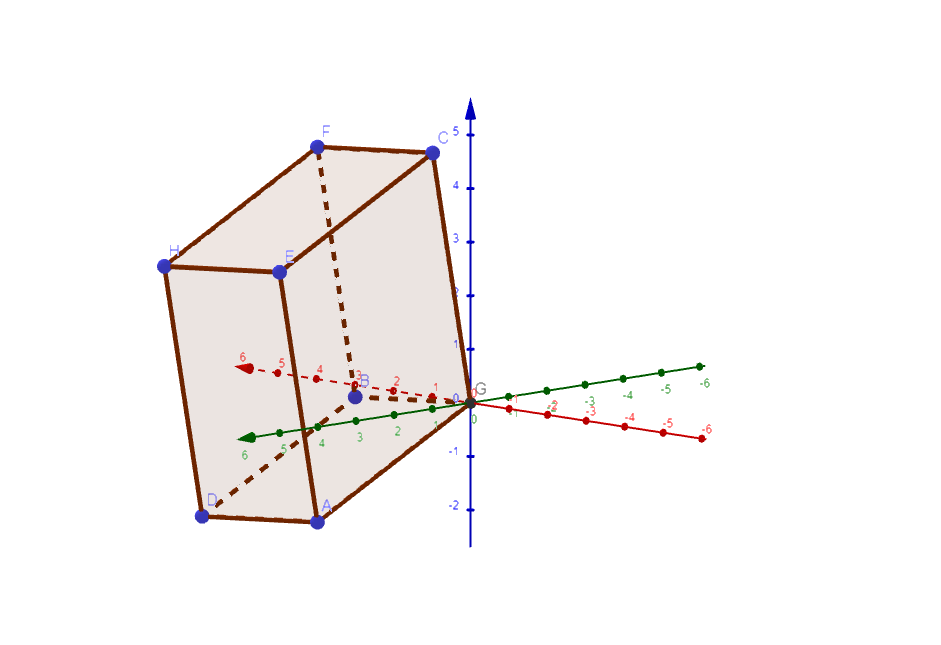
\includegraphics[width=\textwidth]{IntroductionCryptography/exercise-7-7.png}
		\caption{Exercise 7.7 - Fundamental domain of $L$}
	\end{figure}
	$\det (L) = \text{Vol} (\mathcal{F})$


7.43. $t = b_1 b_2 / \lVert b_1 \rVert^2$ and $b_2^* = b_2 - tb_1$ \\ $\Rightarrow b_2^* \cdot b_1 = b_1 (b_2 - tb_1) = b_1 b_2 - t \lVert b_1 \rVert^2 = b_1 b_2 - \frac{b_1 b_2}{\lVert b_1 \rVert^2} \cdot \lVert b_1 \rVert^2 = 0$ \\ Hence $b_2^* \perp b_1$ and $b_2^*$ is the projection of $b_2$ onto the orthogonal complement of $b_1$


7.44.
	
		 $\lVert a - tb \rVert^2 = (a - tb)^2 = a^2 - 2abt + t^2b^2 = \lVert a\rVert^2 + t^2 \lVert b\rVert^2 - 2abt \geq 0$ \\ $\Leftrightarrow a - tb = 0 \Rightarrow t = \frac{ab}{\lVert b \rVert^2}$
		 0
		 $(a - tb)\cdot b = ab - t \lVert b \rVert^2 = ab - \frac{ab}{\lVert b \rVert^2} \cdot \lVert b \rVert^2 = 0$. \\ Therefore $a - tb$ is the projection of $a$ onto the orthogonal complement of $b$
	
7.45.
	\begin{algorithm}[ht]
		\caption{Gauss's latice reduction algorithm}
		\begin{algorithmic}
			\While{True}
				\If{$\lVert v_2 \rVert < \lVert v_1 \rVert$}

				swap $v_1$ and $v_2$	
			
				$m \gets \lfloor v_1 \cdot v_2 / \lVert v_1 \rVert^2 \rceil$
			\EndIf
			\If{$m = 0$}

				return $(v_1, v_2)$
			\EndIf

			Replace $v_2$ with $v_2 - mv_1$
			\EndWhile
		\end{algorithmic}
	
	%\TitleOfAlgo{Gauss's latice reduction algorithm}
	\end{algorithm}
	
		 $v_1 = (14, -47)$, $v_2 = (-362, -131)$, 6 steps
		 $v_1 = (14, -47)$, $v_2 = (-362, -131)$, 6 steps
		 $v_1 = (147, 330)$, $v_2 = (690, -207)$, 7 steps
	


7.46.	
		 $W^\perp$ is the orthogonal complement of $W$ in $V$ $\Rightarrow \vec{z} \in W^\perp$, $\vec{z}\cdot\vec{y} = 0, \forall \vec{y} \in W$ \\ With $\vec{z_1}, \vec{z_2} \in W^\perp \Rightarrow \vec{z_1}\cdot\vec{y} = \vec{z_2}\cdot\vec{y} = 0, \forall \vec{y} \in W$ \\ $\Rightarrow (\vec{z_1} + \vec{z_2})\cdot\vec{y} = 0 \Rightarrow \vec{z_1} + \vec{z_2} \in W^\perp$ \\ $\alpha\vec{z_1}\cdot\vec{y} = \alpha \cdot 0 = 0 \Rightarrow \alpha\vec{z_1} \in W^\perp, \forall \alpha \in \mathbb{R}$
		 We have 2 methods
		
			 \textit{First method}: Show that $W \cup W^\perp = \{\vec{0}\}$. If $\vec{u}$ belongs to both $W$ and $W^\perp$, then $<u, u> = 0 \Rightarrow \vec{u} = \vec{0}$.
			
			Now denote $U = W + W^\perp$, we prove that $W = V$. We can choose an orthonormal basis in $U$ and extend it to orthonormal basis in $V$. Thus, if $U \neq V$, there is an element $\vec{e}$ in the basis of $V$ orthonormal to $U$. Since $U$ contains $W$, $e$ is orthonormal to $U \Rightarrow \vec{e} \in W^\perp$. The latter is a subspace of $W$, therefore $e$ is in $W$, which is contrary.
			 \textit{Second method}: Let $\{e_1, e_2, \cdots, e_k\}$ be an orthonormal basis of the subspace $W$. For each $v \in V$, let $$P(v) = \sum_{j=1}^{k} <v, e_j> e_j$$ $$\Rightarrow (\forall v \in V): v = \underbrace{P(v)}_{\in W} + \underbrace{(v - P(v))}_{\in W^\perp}$$
			The fact that $v - P(v) \in W^\perp$ is: 
			
			if $j \in \{1, 2, \cdots, k\}$ then 
			\begin{align*}
				<v-P(v), e_j> & = <v - \sum_{l=1}^{k}<v, e_l>e_l, e_j> \\
					& = <v, e_j> - <v, e_j> = 0	
			\end{align*}
			Since $\{e_1, \cdots, e_k\}$ is a basic of $W$, this prove that $v-P(v) \in W^\perp$
		
		 $\lVert v \rVert^2 = <v, v> = (aw + bw')^2 = a^2w^2 + 2abww' + b^2w'^2 = a^2 \lVert w \rVert^2 + 0 + b^2 \lVert w' \rVert^2 = a^2 \lVert w \rVert^2 + b^2 \lvert w' \rVert^2$
	



\part{Lịch sử toán học}
Trong lịch sử, từ xa xưa con người đã biết tính toán, sử dụng chúng cho công việc hằng ngày.

Chúng ta không biết ai là người đầu tiên phát minh ra lịch, cũng như cách tính toán để phân chia ruộng đất, tài sản trong các nền văn minh cổ.
Những điều đó được đúc kết theo kinh nghiệm qua hàng chục, thậm chí hàng trăm năm tri thức con người.

Cho tới khi những nhân vật sau (và nhiều nhân vật tương tự khác) đi du lịch Ai Cập và phương đông (ý mình là đi du học).

Đầu tiên phải nhắc tới Euclid, người đã quá quen thuộc với học sinh phổ thông với tiên đề Euclid. Hệ tiên đề Euclid đề ra trở thành cơ sở cho hình học. Bộ sách \textit{Elements} của ông được cho là bộ sách giáo khoa đầu tiên trên thế giới và những gì ghi trong đó khá giống với những gì được giảng dạy ở trường học chúng ta ngày nay.

Nhưng ông đã không lường trước được 1 điều: thế hệ sau đã "thêm mắm dặm muối" và biến đổi hình học của ông thành hình học Phi-Euclid. Từ đó mở ra những khả năng lớn hơn của toán học.

Pythagoras: định lý Pythagoras trong tam giác vuông có lẽ là định lý đầu tiên mà học sinh tiếp cận. Phát biểu rất đơn giản:

\begin{theorem}[Định lý Pythagoras]
    Trong tam giác vuông, bình phương cạnh huyền bằng tổng bình phương hai cạnh góc vuông.

    Nói cách khác, tam giác có 2 cạnh góc vuông lần lượt là $a$ và $b$, cạnh huyền độ dài là $c$ thì
    \[a^2 + b^2 = c^2\]
\end{theorem}

Thật ra trước thời Pythagoras rất lâu, người Ai Cập đã biết tới phương pháp này. Có nhiều bằng chứng về các cuộn giấy papyrus ghi lại các bộ số nguyên $(a, b, c)$ mà $a^2 + b^2 = c^2$ được tìm thấy khi khai quật.

Tuy nhiên thời đó con người chỉ làm việc với các số nguyên, chính xác hơn là các số tự nhiên vì chúng "tự nhiên" xuất hiện trong đời sống.

Pythagoras là người đầu tiên nhắc tới \textbf{proof} (chứng minh) trong toán học. Một phát biểu, định lý chỉ đúng khi có một chứng minh đúng đắn cho nó. Các bước suy luận trong chứng minh dựa trên một hệ tiên đề (axiom) cho trước.
Các tiên đề này hiển nhiên đúng, từ đó các suy luận chính xác sẽ cho kết quả chính xác.

Cho tới khi Fermat phán:

\begin{theorem}[Định lý cuối cùng của Fermat]
    Không tồn tại một cách phân tích tam thừa thành tổng 2 tam thừa, tứ thừa thành tổng 2 tứ thừa, hay tổng quát hơn

    Với mọi số nguyên $n \geq 3$, không tồn tại bộ số nguyên $(a, b, c)$ sao cho
    \[a^n + b^n = c^n\]
\end{theorem}

Và cú lừa có lẽ là lớn nhất thời đại: \textit{"Tôi đã tìm được chứng minh cho mệnh đề kỳ diệu này nhưng lề sách quá chật không thể viết được"}.

Vâng, cái chứng minh kỳ diệu mà ông nói đã khiến các nhà toán học thiên tài bế tắc trong suốt hơn 300 năm, sử dụng nhiều công cụ phức tạp không có ở thời Fermat và hoàn thiện bởi bài báo 200 trang của Andrew Wiles.

Nghĩa là 200 lề sách cũng không viết đủ chứng minh cho định lý cuối cùng của Fermat!!!

Phần này mình làm vì đam mê tìm hiểu lịch sử toán. Ở đây ghi lại cuộc đời và công trình của các nhà toán học lớn trên thế giới suốt chiều dài lịch sử.

Phần này lấy cảm hứng từ quyển \textit{Thiên tài và số phận} và \textit{Định lý cuối cùng của Fermat} của thầy Lê Quang Ánh, thông tin tham khảo dựa trên nhiều nguồn (chủ yếu là quyển \textit{Men of Mathematics} của E.T.Bell).

Tuy nhiên thông tin về cuộc đời của các nhà toán học đã có khá nhiều, mình sẽ trình bày theo cách hiểu của bản thân và đôi khi tập trung nhiều vào các công trình mức cơ sở.

Ngoại trừ phần lịch sử của nhà toán học, mình sẽ trình bày các định lý, khái niệm, ứng dụng của họ theo cách viết, cách trình bày của toán học hiện đại ngày nay để dễ tiếp cận.

\chapter{Euclid}

Lúc mình học cấp 2, tiên đề Euclid được học là một trong 5 tiên đề hình học của Euclid. Nội dung tiên đề đó như sau:

\begin{axiom}[Tiên đề Euclid]
    Qua một điểm nằm ngoài đường thẳng cho trước, ta vẽ được một và chỉ một đường thẳng song song với đường thẳng đã cho.
\end{axiom}

Trong hình học Euclid, hình được vẽ trên \textit{mặt phẳng}. Ở đó, với 2 điểm phân biệt ta vẽ được duy nhất một đường thẳng đi qua 2 điểm đó.

Nếu chúng ta chỉ lấy phần ở giữa 2 điểm, ta có \textit{đoạn thẳng}. Nếu ta lấy phần ở ngoài 2 điểm nhưng chỉ một phía (đường thẳng kéo dài 2 phía) ta có nửa đường thẳng (hay còn gọi là tia).

Chúng ta có 2 công cụ để vẽ hình: thước và compa. Từ 2 công cụ này ta có thể vẽ được rất nhiều hình dạng như chia đôi góc (phân giác), chia đôi cạnh (lấy trung điểm), vẽ đường tròn, đường thẳng.

Tuy nhiên chúng lại có giới hạn: không thể chia 3 góc, hay không thể vẽ được hình đa giác đều 7 cạnh.

Những bài toán nhìn có vẻ đơn giản nhưng phải tới nhiều thế hệ sau, con người mới tìm được cách chứng minh rằng một hình nào đó có dựng được bằng thước và compa hay không.

Tiên đề là những mệnh đề mà ta thừa nhận tính đúng đắn của nó không cần chứng minh. Tuy nhiên sự đúng đắn phải được kiểm nghiệm từ thực tiễn.
Cơ sở của hình học Euclid gồm hệ các tiên đề làm nền móng cho các chứng minh toán học về sau.
\chapter{Zeno}

Zeno là nhà triết học nổi tiếng của Hy Lạp. Trong toán học, ông nổi tiếng về nghịch lý Zeno:

Archiles chạy đua với rùa. Do Archiles chạy nhanh hơn nên sẽ chấp rùa chạy trước. Khi đó Zeno bảo rằng Archiles sẽ không thể đuổi kịp rùa.

Phát biểu nghe rất mâu thuẫn nhưng được Zeno lý giải như sau:

\begin{itemize}[noitemsep]
    \item Giả sử ban đầu Archiles xuất phát sau con rùa một khoảng $d_1$
    \item Archiles mất một khoảng thời gian $t_1$ để đi hết quãng đường $d_1$ đó. Tuy nhiên trong khoảng thời gian $t_1$ đó con rùa cũng đi được một quãng đường $d_2$
    \item Archiles lại mất thêm một khoảng thời gian $t_2$ để đi hết quãng đường $d_2$. Nhưng rùa cũng đã đi được một đoạn $d_3$ nào đó trong thời gian $t_2$ rồi.
    \item Và cứ tiếp tục như thế, ta thấy rằng khoảng cách $d_n$ giữa 2 người sẽ nhỏ dần đi, nhưng không bao giờ chạm 0. Nói cách khác Archiles không thể bắt kịp con rùa.
\end{itemize}

Có gì đó rất \textit{không ổn} ở đây. Rõ ràng trên thực tế Archiles chắc chắn sẽ bắt kịp con rùa trong một khoảng thời gian nhất định. Nhưng tại sao suy luận của Zeno lại cho ra kết quả lạ thường vậy?

Câu trả lời là ở \textbf{vô cực}. Nói theo toán học hiện đại, khoảng cách $d_n$ tiến về 0 khi $n$ tiến ra vô cùng.

Tuy nhiên sự vô cùng chưa được hiểu đúng ở thời của Zeno. Việc này sẽ được giải quyết ở thời của Cantor.
\chapter{Cauchy}

\begin{theorem}[Bất đẳng thức AM-GM]
    Với 2 số không âm $a, b$, ta luôn có
    \[a+b \geq 2 \sqrt{ab}\]
    Dấu bằng xảy ra khi $a = b$.
\end{theorem}

Tổng quát cho $n$ số ta có

\begin{theorem}[Bất đẳng thức AM-GM tổng quát]
    Với $n$ số không âm $a_1, a_2, \ldots, a_n$, ta luôn có
    \[a_1 + a_2 + \ldots + a_n \geq n \sqrt[n]{a_1 a_2 \ldots a_n}\]
    Dấu bằng xảy ra khi $a_1 = a_2 = \ldots = a_n$.
\end{theorem}

Thực tế, bất đẳng thức Cauchy (còn gọi là bất đẳng thức Cauchy-Schwarz) có thể hiểu theo cách cơ bản như sau:

\begin{theorem}[Cauchy-Schwarz]
    Với 2 bộ số $(a_1, a_2, \ldots, a_n)$ và $(b_1, b_2, \ldots, b_n)$ ta có
    \[(a_1^2 + a_2^2 + \ldots + a_n^2) (b_1^2 + b_2^2 + \ldots + b_n^2) \geq (a_1 b_1 + a_2 b_2 + \ldots + a_n b_n)^2\]

    Dấu bằng xảy ra khi $\frac{a_1}{b_1} = \frac{a_2}{b_2} = \ldots = \frac{a_n}{b_n}$
\end{theorem}

Theo ngôn ngữ đại số tuyến tính thì định lý Cauchy-Schwarz như sau:

\begin{theorem}[Cauchy-Schwarz]
    Trong không gian Euclid, với mọi vector $\vec{x}$ và $\vec{y}$ thì 
    \[\lVert \vec{x} \rVert \cdot \lVert \vec{y} \rVert \geq \langle \vec{x}, \vec{y} \rangle\]
    
    Có nghĩa là, tích độ dài 2 vector bất kì lớn hơn hoặc bằng tích vô hướng của chúng.

    Dấu bằng xảy ra khi 2 vector đó cùng phương.
\end{theorem}
\chapter{Nicolai Ivanovich Lobachevsky}

Nhà toán học vĩ đại người Nga 
\begin{otherlanguage}{russian}
    Лобачевский Николай Иванович   
\end{otherlanguage}
(N.I. Lobachevsky) (1792-1856) là người có công rất lớn trong việc xây dựng hình học phi Euclid.



\part{Mật mã học}
\documentclass{article}

\usepackage{geometry}
\usepackage[utf8]{inputenc, vietnam}
\usepackage{amsmath, amsfonts}

\geometry{a5paper}

\title{Về Mix Column trong AES}
\author{Lê Quốc Dũng}

\begin{document}

Giả sử ma trận trạng thái trước khi bước vào phép tính Mix Column của AES
là 
\begin{equation}
    \begin{pmatrix}
        c_0 & c_1 & c_2 & c_3 \\
        c_4 & c_5 & c_6 & c_7 \\
        c_8 & c_9 & c_{10} & c_{11} \\
        c_{12} & c_{13} & c_{14} & c_{15}
    \end{pmatrix}
\end{equation}

Phép tính Mix Column lấy mỗi cột của ma trận trạng thái trên làm tham số cho đa thức
với hệ số trong $GF(2^8)$ và nhân với đa thức $c(z) = 2 + z + z^2 + 3z^3$ rồi modulo
cho $z^4 + 1$.

Giả sử với cột đầu tiên, ta viết hệ số theo thứ tự bậc tăng dần
$d(z) = c_0 + c_4 z + c_8 z^2 + c_{12} z^3$.

Tính (trong $GF(2^8)$)

\begin{align*}
    c(z) \cdot d(z) = & (2 + z + z^2 + 3 z^3) \cdot (c_0 + c_4 z + c_8 z^2 + c_{12} z^3) \\
    = & 2 c_0 + 2 c_4 z + 2 c_8 z^2 + 2 c_{12} z^3 \\
    + & c_0 z + c_4 z^2 + c_8 z^3 + c_{12} z^4 \\
    + & c_0 z^2 + c_4 z^3 + c_8 z^4 + c_{12} z^5 \\
    + & 3 c_0 z^3 + 3 c_4 z^4 + 3 c_8 z^5 + 3 c_{12} z^6 \\
    = & 2 c_0 + (2 c_4 + c_0) z + (2 c_8 + c_4 + c_0) z^2 \\
    + & (2 c_{12} + c_8 + c_4 + 3 c_0) z^3 + (c_{12} + c_8 + 3 c_4) z^4 \\
    + & (c_{12} + 3 c_8) z^5 + 3 c_{12} z^6
\end{align*}

Trong $GF(2^8)$ thì mọi phần tử đều có tính chất $2 x^n = 0$, tương đương với
$x^n = -x^n$. Do đó 
\begin{align*}
    & z^6 \pmod{z^4 + 1} \equiv -z^2 \equiv z^2 \\
    & z^5 \pmod{z^4 + 1} \equiv -z \equiv z \\
    & z^4 \pmod{z^4 + 1} \equiv -1 \equiv 1
\end{align*}

Suy ra
\begin{align*}
    c(z) \cdot d(z) = & 2 c_0 + (2 c_4 + c_0) z + (2 c_8 + c_4 + c_0) z^2 \\
    + & (2 c_{12} + c_8 + c_4 + 3 c_0) z^3 + (c_{12} + c_8 + 3 c_4) \\
    + & (c_{12} + 3 c_8) z + 3 c_{12} z^2 \\
    = & (c_{12} + c_8 + 3 c_4 + 2 c_0) + (c_{12} + 3 c_8 + 2 c_4 + c_0) z \\
    + & (3 c_{12} + 2 c_8 + c_4 + c_0) z^2 + (2 c_{12} + c_8 + c_4 + 3 c_0) z^3
\end{align*}

Như vậy xét hệ số lần lượt trước 1, $z$, $z^2$ và $z^3$ thì tương đương với phép
nhân ma trận

\begin{equation}
    \begin{pmatrix}
        2 & 3 & 1 & 1 \\
        1 & 2 & 3 & 1 \\
        1 & 1 & 2 & 3 \\
        3 & 1 & 1 & 2
    \end{pmatrix} \cdot
    \begin{pmatrix}
        c_0 \\ c_4 \\ c_8 \\ c_{12}
    \end{pmatrix}
\end{equation}
\end{document}

\medskip

\bibliography{mybib}

\end{document}